\documentclass[10pt]{scrartcl}

\usepackage[bluelinks]{drangreport}
% \usepackage[caecilia]{drangreport}

\def\n{5}
\def\m{4}


\renewcommand{\theequation}{\arabic{equation}}


\hypersetup{pdfinfo={
Title={M1P2: Algebra I Lecture Notes},
Author={Karim Bacchus},
Keywords ={Algebra I, M1P2, Lecture Notes, Imperial College, Maths},
}}


\title{Algebra I}

\begin{document}

\NotesSubTitle{1st}{Spring 2015}{Algebra I}{Dr.~J. R.}{Britnell}
{


\subsection*{Syllabus}

\textit{Introductions to three topics in abstract algebra: The theory of vector spaces and linear
transformations, the theory of groups and the theory of rings.}


\emph{Vector spaces:} Linear maps, rank-nullity theorem, connections with linear equations and matrices.

\emph{Groups:} Axioms, examples. Cyclic groups, dihedral groups, symmetric groups. Lagrange’s  theorem and applications.

\emph{Rings:}  Polynomial rings, rings of the form Z[$\sqrt{d}$]. Euclid’s algorithm for certain rings. Uniqueness of factorisation for these rings. Applications to Diophantine Equations.


\subsection*{Appropriate books}

{\shortskip
J.~Fraleigh and R.~Beauregard, \emph{Linear Algebra}

S.~Lipschutz and M.~Lipson, \emph{Linear Algebra}

J.~B.~Fraleigh, \emph{A First Course in Abstract Algebra}

R.~Allenby, \emph{Rings, Fields and Groups}

I.~N.~Herstein, \emph{Topics in Algebra}
}}

\TableofContents

%!TEX root = M1P2.tex

\stepcounter{lecture}
\setcounter{lecture}{1}
\pagebreak
\addcontentsline{toc}{part}{Linear Algebra}{}
\setcounter{page}{3}
\sektion{Vector Spaces}

\subsektion{Spanning Sets and Bases (M1GLA Review)}
Let \lecturemarker{1}{15 Jan}  $V$ be a vector space, and let $S = \{v_1, \dots, v_k\}$ be a finite subset of $V$. Then the \emph{span}\index{Span} of $S$ is the set $\{\lambda_1v_1 + \lambda_2v_2 + \dots + \lambda_kv_k, \lambda_1,\dots,\lambda_k \text{ scalar}\}.$

\begin{itemize}
\item[*] Span $S$ is a subspace of $V$.
\item[*] If Span $S = V$, then we say that $S$ is a \emph{spanning set}\index{Spanning Set} for $V$. 
\item[*] If $V$ has a finite spanning set, then we say that $V$ is finite dimensional.
\end{itemize}


Assume from now on that $V$ is finite dimensional. The set $S$ is \emph{linearly independent}\index{Linear Independence} if the only solution to the equation $\lambda_1v_1 + \lambda_2v_2 + \dots + \lambda_kv_k = \mathbf{0}$ is $\lambda_1 = \lambda_2 = \dots = \lambda_k = 0.$\\

A \emph{basis}\index{Basis} for $V$ is a linearly independent spanning set.

\begin{itemize}
\item[*] $V$ has a basis
\item[*] Every basis of $V$ has the same size. This is the \emph{dimension}\index{Dimension} of $V$, written dim $V$. 
\end{itemize}

Suppose that dim $V = n$.
\begin{itemize}
\item[*] Any spanning set of size $n$ is a basis. 
\item[*] Any linearly independent set of size $n$ is a basis.
\item[*] Every spanning set contains a basis as a subset.
\item[*] Every linearly independent set is contained as a subset in a basis.
\item[*] Any subset of $V$ of size $< n$ is \textbf{not} a spanning set.
\item[*] Any subset of $V$ of size $>n$ is \textbf{not} linearly independent. 
\item[*] If $W$ is a subspace of $V$ then dim $W \leq $ dim $V$ eith equality only when $W = V$. 
\end{itemize}\vspace*{5pt}

Every vector space has associated with it a set of \emph{scalars}. E.g. $\mathbb{R}^n$ has the scalar set $\mathbb{R}.$ The scalars come as a structure called a \emph{field} (To be defined in the Ring Theory Section). I'll write $F$ for the field of scalars. It will usually be safe to assume that $F = \mathbb{R}$. Other fields include $\mathbb{C}, \mathbb{Q}$, integers and $(\mathbb{Z}\backslash p \mathbb{Z})^{\times}$.

\subsektion{More on Subspaces}\vspace*{5pt}

\begin{definition} Let $V$ be a vector space, and let $U$ and $W$ be subspaces of $V$. The \emph{intersection}\index{Intersection} of $U$ and $W$ is $U \cap W = \{v: v \in U \text{ and } v \in W\}$. The \emph{subspace sum}\index{Subspace Sum} (or just \emph{sum}) of $U$ and $W$ is $U + W = \{u + w: u \in U, w \in W\}$
\end{definition}\vspace*{5pt}

\begin{remark}  Note that $\mathbf{0} \in U$ and $\mathbf{0} \in W$, so if $u \in U$, then $u = \mathbf{0} \in U + W$, and similarly if  $w \in W$, then $w = \mathbf{0} \in U + W$. So $U \subseteq U + W$ and $W \subseteq U + W$. ($U+W$ usually contains many other vectors)
\end{remark}\vspace*{10pt}

\begin{example} Let $V \in \mathbb{R}^2.$ Let $U = \text{Span}\{(1,0)\}$, and  $W = \text{Span}\{(0,1)\}$. So $U = \{(\lambda, 0): \lambda \in \mathbb{R}\}, ~W = \{(0,\lambda: \lambda \in \mathbb{R}\}$. We see that $U + W$ contains $(\lambda, \mu)$ for all $\lambda, \mu \in \mathbb{R}$ and so $U + W = V$.
\end{example}\vspace*{5pt}



\begin{proposition} $U \cap W$ and $U + W$ are both subspaces of $V$. 	
\end{proposition}

\begin{proof}
Do $U+W$ first. Checking the subspace axioms:
\begin{enumerate}
\item  $\mathbf{0} \in U$ and $\mathbf{0} \in W \implies \mathbf{0} = \mathbf{0} + \mathbf{0} \in U + W$. So $U + W \neq \emptyset$. 
\item Suppose $v_1, v_2 \in U + W$. Then $v_1 = u_1 + w_1$ and $v_2 = u_2 + w_2,$ where $u_1,u_2 \in U$ and $w_1, w_2 \in W$.\\

Now $v_1 + v_2 = u_1 + w_1 + u_2 + w_2 = (u_1 + u_2) + (w_1 + w_2) \in U + W \implies$ closed under addition.

\item Let $v \in U + W$. Then $v = u + w$ where $u \in U$ and $w \in W.$ Let $\lambda \in F$. Then $\lambda v = \lambda(u+w) = \lambda u + \lambda w \in U + W$.
\end{enumerate}

Now do $U \cap W$:
\begin{enumerate}
\item $\mathbf{0} \in U$ and $\mathbf{0} \in W$, so $\mathbf{0} \in U \cap W$ by definition.
\item Suppose $v_1, v_2 \in U \cap W.$ Then $v_1, v_2 \in U$ and so $v_1 + v_2 \in U$ since $U$ is closed. Similarly for $v_1 + v_2 \in W$. Hence $v_1 + v_2 \in U \cap W$. 
\item Suppose $v \in U \cap W$, and $\lambda \in F.$ Then $v \in U$ and so $\lambda v \in U$. $v \in W \implies \lambda v \in W.$ Hence $\lambda v \in U \cap W$.\qedhere 
\end{enumerate}
\end{proof}\vspace*{10pt}

\begin{proposition}Let {\normalfont\lecturemarker{2}{5 oct}}
 $V$ be a vector space and let $U ~\&~ W$ be subspaces. Suppose that $U = \text{Span}\{u_1,\dots,u_r\}$ and $W = \text{Span}\{w_1,\dots,w_s\}$. Then $U + W = \text{Span}\{u_1,\dots,u_r,w_1,\dots,w_s\}$. 
\end{proposition}
\begin{proof}
By inclusion both ways:

Notice that $u_i \in U \subseteq U + W$ (by Remark 2) and similarly $w_i \in W \subseteq U + W, ~\forall i$. Since $U + W$ is a subspace of $V$, so $U + W$ is closed under linear combinations, so $\text{Span}\{u_1,\dots,u_r,w_1,\dots,w_s\} \subseteq U + W.$

For the reverse inclusion, let $v \in U + W$. Then $v = u + w$ for some $u \in U, w \in W$. Since $U = \text{Span}\{u_1,\dots,u_r\}$, we have $u = \lambda_1u_1 + \dots + \lambda_ru_r$, for some $\lambda_1,\dots,\lambda_r \in F$. Similarly $w = \mu_1w_1 + \dots + \mu_sw_s$, for some $\mu_1,\dots,\mu_s \in F$.

Now $v = \lambda_1u_1 \dots \lambda_ru_r + \mu_1w_1 \dots \mu_sw_s \in \text{Span}\{u_1,\dots,u_r,w_1,\dots,w_s\}$. Hence $U + W \subseteq \text{Span}\{u_1,\dots,u_r,w_1,\dots,w_s\}$.
\end{proof}\vspace*{5pt}

\begin{examples}\item \textbf{Question:} 
 Let $V = \mathbb{R}^4, U = \text{Span}\{(1,1,2,-3),(1,2,0,-3)\}$  and\\ $W = \text{Span}\{(1,0,5,-4),(-1-3,0,5)\}.$ Find a basis for $U + W.$ 

\textbf{Answer:} By Proposition 5, we have:
 \[U + W = \text{Span}\{(1,1,2,-3),(1,2,0,-3),(1,0,5,-4),(-1,-3,0,5)\}\] 
 
 We then just row reduce the matrix:
 
 \[\begin{pmatrix}
 1 & 1 & 2 & -3\\
 1 & 2 & 0 & -3\\
 1 & 0 & 5 & -4\\
 -1 & -3 & 0 & 5
 \end{pmatrix} \rightarrow \textit{Echelon Stuff} \rightarrow
 \begin{pmatrix}
 1 & 1 & 2 & -3\\
 0 & 1 &-2 & 0\\
 0 & 0 & 1 & -1\\
 0 & 0 & 0 & 0
 \end{pmatrix}  \]

The three non-zero rows are linearly independent, and have the same span as the original four vectors, so a basis for $U + W$ is:
\[\{(1,1,2,-3),(0,1,-2,0),(0,0,1,-1)\} \text{ (or just the first 3 vectors).}\]

\item \textbf{Question:} What about a basis for $U \cap W$?

\textbf{Answer:} If $v \in U \cap W$, then $v \in U = \text{Span}\{(1,1,2,-3),(1,2,0,-3)\}.$ So $v = a(1,1,2,-3) + b(1,2,0,-3)$ for $a,b \in \mathbb{R}$. And $v \in W = \text{Span}\{(1,0,5,-4),(-1,-3,0,5)\}$. So $v = c(1,0,5,-4) + d(-1,-3,0,5)$. So we have:
\[a(1,1,2,-3) + b(1,2,0,-3) -c(1,0,5,-4) -d(-1,3,0,5) = \mathbf{0} ~(*)\]

$(*)$ gives us 4 simultaneous equations, which we can encode as a matrix equation:
\[
\begin{pmatrix}
1 & 1 & -1 & 1\\
1 & 2 & 0 & -3\\
2 & 0 & -5 & 0\\
-3 & -3 & 4 & -5
\end{pmatrix}
\begin{pmatrix}
a\\b\\c\\d
\end{pmatrix}
=
\mathbf{0} \]

We find the solution space by row reducing:
\[
\begin{pmatrix}
1 & 1 & -1 & 1\\
1 & 2 & 0 & -3\\
2 & 0 & -5 & 0\\
-3 & -3 & 4 & -5
\end{pmatrix} \rightarrow \textit{Echelon Stuff} \rightarrow
 \begin{pmatrix}
 1 & 0 & 0 & -5\\
 0 & 1 & 0 & 4\\
 0 & 0 & 1 & -2\\
 0 & 0 & 0 & 0
 \end{pmatrix}  \]

There is one line of solutions, given by $a = 5d, b = -4d, c = 2d.$ So pick $d = 1$, then $a = 5, b = -4, c = 2, d =1$. So \[v = a(1,1,2,-3) + b(1,2,0,-3) = (5,5,10,-15) - (4,8,0,-12) = (1,-3,10,3)\]
We can check our solutions with $c,d$: $v = c(1,0,5,-4) + d(-1,-3,0,5) = (1,-3,10,3)$ as expected. So $U \cap W$ is 1-dimensional, and a basis is $\{(1,-3,10,3)\}$.
\end{examples}


\begin{theorem} Let $V$ be a vector space, and let $U$ and $W$ be subspaces. Then dim $U + W = $ dim $U + $ dim $W - $ dim $U \cap W$.	
\end{theorem}


\begin{proof}
Let dim $U = r, $ dim $W = s, $ dim $U \cap W = m$. Let $\{v_1, \dots, v_m\}$ be a basis for $U \cap W$. Then $\{v_1,\dots,v_m\}$ is a linearly independent subset of $U$. So it is contained in some basis for $U$. So there exists $u_1,\dots, u_{r-m}$ in $U$ such that $\{v_1,\dots,v_m,u_1,\dots,u_{r-m}\}$ is a basis for $U$. Similarly, there exists $w_1,\dots,w_{s-m}$ such that $\{v_1,\dots,v_m,w_1,\dots,w_{s-m}\}$.

Now let $B = \{v_1,\dots,v_m,u_1,\dots,u_{r-m},w_1,\dots,w_{s-m}\}$. Then Span $B = U + W$ by Proposition 5.

\textbf{Claim.} $B$ is linearly independent.

Proof of claim:

Suppose that $\alpha_1v_1 + \dots \alpha_mv_m + \beta_1u_1 + \dots \beta_{r-m}u_{r-m} + \gamma_1w_1 + \dots \gamma_{s-m}w_{s-m} = \mathbf{0}.$ For $\alpha_i, \beta_i, \gamma_i \in F$. Then:

\[\sum_{i=1}^{s-m} \gamma_iw_i = -\sum_{i = 1}^{m} \alpha_iv_i - \sum_{i=1}^{r-m} \beta_iu_i \in U \]

\[\implies \sum_{i=1}^{s-m} \in U \cap W \implies \sum_{i=1}^{s-m} = \sum_{i=1}^{m} \delta_iv_i, \text{ for some } \delta_i \in F\]

\[\text{Hence:~ }\sum_{i=1}^{m} \delta_iv_i - \sum_{i=1}^{s-m} \gamma_iw_i = \mathbf{0}.\]

But $\{v_1,\dots,v_m,w_1,\dots,w_{s-m}\}$ is linearly independent (being a basis for $W$). So $\gamma_i =\delta_i = 0, \forall i$. Since $\gamma_i = 0 ~\forall i$, we have:

\[\sum_{i=1}^{m} \alpha_iv_i + \sum_{i=1}^{r-m} \beta_iu_i = \mathbf{0}.\]
 
 But $\{v_1,\dots,v_m,u_1,\dots,u_{r-m}\}$ is linearly independent (being a basis for $U$). So $\alpha_i =\beta_i = 0, \forall i$. Hence $B$ is linearly independent. So $B$ is a basis for $U+V$. So dim $U + W = |B| = m + (r-m) + (s-m) = r + s - m$.
\end{proof}\vspace*{10pt}
 
\begin{example} \textbf{Question:} \lecturemarker{3}{20/01} 
 Let $V = \mathbb{R}^3$, and let $U= \{(x,y,z) \in \mathbb{R}^3: x + y + z = 0\}.$ Similarly let $W = \{(x,y,z) \in \mathbb{R}^3: -x + 2y + z = 0\}.$ Find bases for $U, W, U \cap W, U + W$. 

\textbf{Answer:} A general element of $U$ is $(x,y,-x-y) = x(1,0,-1) + y(0,1,-1) \implies U = \text{Span}\{(1,0,-1),(0,1,-1)\}$. Since this set is clearly linearly independent, it's a basis for $U$. A general element of $W$ is $(x,y,x-2y) = x(1,0,1) + y(0,1,-2) \implies W = \text{Span}\{(1,0,1),(0,1,-2)\}$. Again, clearly linearly independent, so a basis for $W$.

Suppose that $v = (x,y,z)$ lies in $U \cap W$. Then $v \in U$, and so $z = -x-y$. But also $v \in W$, and so $z = x - 2y$. Hence $-x-y = x-2y \implies y = 2x$. So a general element of $U \cap W$ is $(x,2x,-3x) = x(1,2,-3) \implies U\cap W = \{(1,2,-3)\} $ is a basis for $U\cap W$.


As in the proof of theorem 7, we find a basis for $U$, and $W$, each of which contain a basis for $U \cap W$. So any linearly independent subset of $U$ of size 2 is a basis for $U$, i.e. $U = \{(1,2,-3),(1,0,-1)\}$. Similarly $W = \{(1,2,-3),(1,0,1)\} $. So a spanning set for $U + W = \{(1,2,-3),(1,0,-1),(1,0,1)\}$.

By Theorem 7, we know dim $U+W = $ dim $U + $ dim $W - $ dim $U\cap W = 2 + 2 -1 = 3.$ Hence our spanning set is a basis for $U + W$.
\end{example}\vspace*{5pt}


\subsektion{Rank of a Matrix}\vspace*{5pt}

\begin{definition}Let $A$ be an $m \times n$ matrix with entries from $F$. Define the \emph{row-span}\index{Row-Span} of $A$ by $\text{RSp}(A) = \text{Span}\{\text{rows of }A\}$. This is a subspace of $F^n$. The \emph{column-span}, $\text{CSp}(A)$ of $A$ is  $\text{Span}\{\text{columns of }A\}$, again a subspace of $F^n$.	

The \emph{row-rank}\index{Row-Rank} of $A$ is dim $\text{RSp}(A)$.I The \emph{column-rank} of $A$ is dim $\text{CSp}(A)$ i.e. the number of linearly independent rows / columns.
\end{definition}\vspace*{5pt}


\begin{example}
$A = \begin{pmatrix}
 3 & 1 & 2\\
 0 & -1 & 1
 \end{pmatrix},~ F = \mathbb{R}$\\
 
 $\text{RSp}(A) = \text{Span}\{(3,1,2),(0,-1,1)\}$. Since the two vectors are linearly independent, we have that the row-rank = dim $\text{RSp}(A) = 2$.\\
 
 $\text{CSp}(A) = \text{Span}\left\{
 \begin{pmatrix}
 3\\0 
 \end{pmatrix}, 
 \begin{pmatrix}
 1 \\ -1
 \end{pmatrix},
 \begin{pmatrix}
 2\\1
 \end{pmatrix}
\right\}$. \\

This is linearly dependent, since $
\begin{pmatrix}
3\\0
\end{pmatrix}
= 
\begin{pmatrix}
1\\-1
\end{pmatrix}
+ \begin{pmatrix}
 2\\1
 \end{pmatrix}
$.\\~\\

So $\text{CSp}(A) = \text{Span}\left\{
\begin{pmatrix}
 1 \\ -1
 \end{pmatrix},
 \begin{pmatrix}
 2\\1
 \end{pmatrix}
\right\} \implies \text{CSp}(A) = 2.$
\end{example}



\textit{How do we calculate the row-rank of a matrix $A$?}\\


\begin{proc}~\\

\noindent \textbf{Step 1:} Use row operations to reduce the matrix $A$, to row echelon form.

\[A_{ech} =\left(
    \begin{array}{ccccc}
    1    &       &    &     & \\ \cline{1-1}
    \bord & 1       &    &  \scalebox{1.5}{*}   & \\ \cline{2-2}
          & \bord    & 1     &    & \\ \cline{3-3}
       ~\scalebox{1.5}{0}   &  & \bord & 1     &  \\ \cline{4-5}
          &          &       &  &  \\ %\cline{5-5}
  \end{array}\right)\]

\noindent \textbf{Step 2:} The row-rank of $A$ is the number of non-zero rows in $A_{ech}$, and the non-zero rows of $A_{ech}$ form a basis for $\text{RSp}(A).$ [i.e. you don't need to go back to original vectors get the basis.]
\end{proc}

\textbf{Justification} We need to show:
\begin{enumerate}
\item $\text{RSp}(A) = \text{RSp}(A_{ech})$
\item The non-zero rows of $A_{ech}$ are linearly independent. 
\end{enumerate}

To show (1), recall that $A_{ech}$ is obtained from $A$ by a series of row-operations:
\[
\begin{cases}
r_i := r_i + \lambda r_j & (i\neq j)\\
r_i := \lambda r_i & (\lambda \neq 0)\\
r_i \longleftrightarrow r_j & (i \neq j)
\end{cases} \]

Suppose that $A'$ is obtained from $A$ by one row-operation. Then it is clear than every row of $A'$ lies in $\text{RSp}(A)$. So $\text{RSp}(A') \subseteq \text{RSp}(A)$. But every row operation is invertible by another row operation. i.e. 

\[\begin{cases}
r_i := r_i + \lambda r_j & \text{has inverse ~} r_i := r_i - \lambda r_j \\
r_i := \lambda r_i & \text{has inverse ~} r_i := r_i - 1/\lambda r_j \\
r_i \longleftrightarrow r_j & \text{has inverse ~}  r_i \longleftrightarrow r_j
\end{cases} \]

So we have $\text{RSp}(A) \subseteq \text{RSp}(A')$, and so the row spaces are equal. It follows that $\text{RSp}(A_{ech}) = \text{RSp}(A)$.

For (2), consider the form of $A_{ech},$ and denote $r_1,\dots r_k$ as the non-zero rows. Say $r_i$ has it's leading entry in column $c_i$. Suppose that \[\lambda_1r_1 + \dots + \lambda_kr_k = \mathbf{0} \tag{$*$}\]
  Look at the co-ordinate corresponding to column $c_1$. The only contribution is $\lambda_1r_1$ since all of the other rows have 0 in that co-ordinate. Since $r_1$ has 1 in this co-ordinate $\implies \lambda_1 = 0$. Since $\lambda_1 = 0$, the only contribution to $c_2$ is $\lambda_2r_2$. So $\lambda_2 = 0$. We can continue this argument for $c_2, \dots, c_i, \dots, c_k \implies$ the only solution to $(*)$ is $\lambda_1, \dots, \lambda_k = 0 \implies $ linearly independence of vectors.\\
  

\begin{example} \lecturemarker{4}{21 Jan} 
Find the row-rank of $A = \begin{pmatrix}
 1 & 2 & 5\\ 2 & 1 & 0 \\ -1& 4 & 15
 \end{pmatrix}
$ \\

\noindent \textbf{Answer:} Reduce $A$ to echelon form: 

\[A  = \begin{pmatrix}
 1 & 2 & 5\\ 2 & 1 & 0 \\ -1& 4 & 15
 \end{pmatrix} \to \begin{pmatrix}
1 & 2 & 5 \\ 0 & 1 & 10/3 \\ 0 & 0 & 0
\end{pmatrix} = A_{ech}\]

Since $A_{ech}$ has two non-zero rows, the row-rank of $A$ is 2. (Note: Scaling the second row to make the leading entry 1 was not necessary)
\end{example}\vspace*{10pt}

\begin{example} Find the dimension of $W = \text{Span}\{(-1,1,0,1),(2,3,1,0),$\\$(0,1,2,3)\} \subseteq \mathbb{R}^4$

 \textbf{Answer:} Notice that $W = \text{RSp} \begin{pmatrix}
 -1 & 1 & 0 & 1\\ 2 & 3 & 1 & 0\\ 0 & 1 & 2 & 3
 \end{pmatrix} = A$
 
 \[\implies A_{ech} =  
 \begin{pmatrix}
 -1 & 1 & 0 & 1 \\ 0 & 5 & 1 & 2 \\ 0 & 0 & 9 & 12
 \end{pmatrix}\]
 
There are 3 non-zero rows in $A_{ech}$, so the row rank is 3. Hence dim $W = 3$.
\end{example}\vspace*{5pt}

\begin{proc}The columns of $A$ are the rows of $A^T$. So apply Procedure 11 to the matrix $A^T$. (Alternatively, use column operations to reduce $A$ to ``column echelon form'', and then count the no. of non-zero columns).\end{proc}

\begin{example} Let $A = \begin{pmatrix}
 1 & 2 & 5\\ 2 & 1 & 0\\ -1 &4 & 15
 \end{pmatrix}
 $\\
 
 The column rank of $A$ is the row-rank of $A^T$.
 
 \[A^T = \begin{pmatrix}
 1 & 2 & -1\\ 2 & 1 & 4\\ 5 & 0 & 15
 \end{pmatrix}
 \to 
 \begin{pmatrix}
 1 & 2 & -1\\ 0 & -3 & 6\\ 0 & 0 & 0
 \end{pmatrix}\]
 
 There are two non-zero rows, so row-rank($A^T$) = 2, and so column-rank $(A)$ = 2. A basis for $\text{RSp}(A^T)$ is $\{(1,2,-1),(0,-3,6)\}$, so a basis for $\text{CSp}(A)$ is the transpose of these vectors.
 \end{example}
 
\begin{theorem} For any matrix $A$, the row-rank of $A$ is equal to the column-rank of $A$.\end{theorem}
 
 \begin{proof}
 Let the rows of $A$ be $r_1, \dots, r_m$, so $r_i = (a_{i1}, a_{i2},\dots,a_{in})$.\\
 
 Let the columns of $A$ be $c_1,\dots,c_n$, so $c_j = (a_{1j}, a_{2j},\dots,a_{mj})^T$.\\
 
 Let $k$ be row-rank of $A$. Then $\text{RSp}(A)$ has basis $\{v_1,\dots,v_k\}, v_i \in F^n$. Every row $r_i$ is a linear combination of $v_1,\dots,v_k$. Say that:
 \[r_i = \lambda_{i1}v_1 + \lambda_{i2}v_2 + \dots + \lambda_{il}v_k ~(*)\]
 
 Let $v_i = (b_{i1}, \dots, b_{in})$. Looking at the $j$th co-ordinate in $(*)$, we have $a_{ij} = \lambda_{i1}b_{1j} + \lambda_{i2}b{2j} + \dots + \lambda_{ik}b_{kj}$
 
 \[c_j = \begin{pmatrix}
 a_{1j}\\a_{2j}\\ ... \\ a_{mj}
\end{pmatrix}
= 
\begin{pmatrix}
\lambda_{11}b_{1j} + \lambda_{12}b_{2j} + \dots + \lambda_{1k}b_{kj}\\
\lambda_{21}b_{2j} + \lambda_{22}b_{2j} + \dots + \lambda_{2k}b_{kj}\\
\dots \\
\lambda_{m1}b_{1j} + \lambda_{m2}b_{2j} + \dots + \lambda_{mk}b_{kj}\\
\end{pmatrix}\]~

So every column of $A$ is a linear combination of $(\lambda_{1i},\lambda_{2i},\dots,\lambda_{mi})^T$ for $1 \leq i \leq k$. So the column space of $A$ is spanned by $k$ vectors and so column-rank$(A) \leq k = $ row-rank$(A)$. But row-rank$(A$) = column-rank($A^T)$, column-rank($A)$ = row-rank($A^T$). 

By the argument above, column-rank$(A^T) \leq$ row-rank($A$). So row-rank$(A) \leq$ column-rank($A$). Hence row-rank$(A)$ = column-rank$(A$).
 \end{proof}\vspace*{5pt}

 
\begin{definition} Let $A$ be matrix. The \emph{rank}\index{Rank} of $A$, written $rk(A)$, is the row-rank of $A$. (which is also the column-rank of $(A$).)	
\end{definition}\vspace*{10pt}


\begin{example}Let $A = \left(\begin{smallmatrix}
 1 & 2 & -1 & 0\\ -1 & 1 & 0 & 1\\ 0 & 3 & -1 & 1
 \end{smallmatrix}\right)$\\
 
 Notice that $r_3 = r_1 + r_2$. So a basis for $RSp(A)$ is $\{(1,2,-1,0),(-1,1,0,1)\}$
 
 Write the rows of $A$ as linear combinations of $\{v_1,v_2\}$:
 \[r_1 = 1v_1 + 0v_2~~~ r_2 = 0v_1 + 1v_2~~~ r_3 = 1v_1 + 1v_2\] (The scalars here are the $\lambda_{ij}$ from the proof of Theorem 16)
 
 According to the proof, a spanning set of for $CSp(A)$ is given by: \[\{(1,0,1)^T,(0,1,1)^T\}\] We verify this - 
 We have $c_1 = (1,-1,0)^T = w_1 - w_2$. $c_2 = (2,1,3)^T = 2w_1 + w_2$, $c_3 = (-1,0,-1)^T = -w_1$, and $c_4 = (0,1,1)^T = w_2$.
 \end{example}\vspace*{5pt}

\begin{proposition} {\normalfont\lecturemarker{5}{23/01} }
 Let $A$ be an $n \times n$ (square) matrix. Then the following statements are equivalent:
\begin{enumerate}
\item $rk(A) = n$ (A has ``full rank'')
\item The rows of $A$ form a basis for $F^n$
\item The columns of $A$ form a basis of $F^n$
\item A is invertible (so det$A \neq 0$, row reduced to $I$ etc.)
\end{enumerate}
\end{proposition}

\begin{proof}
(1) $\iff$ (2):\\
\[\begin{aligned}
\text{rk}(A) = n & \iff \text{dim RSp}(A) = n\\
&\iff \text{RSp}(A) = F^n\\
& \iff \text{Rows of } A \text{ are spanning a set for } F^n \text{ of size } n\\
& \iff \text{The rows of } A \text{ form a basis for }F^n
\end{aligned}
\]

(1) $\iff$ (3): The same, using columns instead.\\

(1) $\iff$ (4): 
\begin{align*}
\text{rk}(A) = n &\iff A_{ech} = I\\
&\iff A \text{ can be row-reduced to } I\\
&\iff A \text{ is invertible.}	\qedhere
\end{align*}
\end{proof}

\subsektion{Linear Transformations}
Suppose that $V$ and $W$ are vector spaces over a field $F$. Let $T: V \to W$ be a function.

\begin{itemize}
\item[*] Say that $T$ ``preserves addition'', if whenever $T: V \mapsto W$ and $T: v_2 \mapsto w_2$, we also have $T: v_1 + v_2 \mapsto w_1 + w_2$. (Briefly: $T(v_1 + v_2)=Tv_1 +Tv_2$.)
\item[*] Say that $T$ ``preserves scalar multiplcation'', if whenever $T: v \mapsto w$ and $\lambda \in F \implies T: \lambda v \mapsto \lambda w$. (Briefly: $T(\lambda v) = \lambda T(v))$
\end{itemize}\vspace*{5pt}

\begin{definition}The function $T: V \to W$ is a \emph{linear transformation}\index{Linear Transformation} (or \emph{linear map}), if it preserves addition and scalar multiplication. So:
\[T(v_1 + v_2)=Tv_1 +Tv_2 \text{ and }T(\lambda v) = \lambda(T(v)), \forall v_1,v_2,v \in V ~\&~ \lambda \in F\]
\end{definition}\vspace*{10pt}


\begin{examples}
\begin{itemize}
\item[(a)] $T: \mathbb{R}^2 \to \mathbb{R}, T(x,y) = x+y$. I claim this is a linear transformation.\\
Check it preserves addition: \[
\begin{aligned}
T( (x_1, y_1) + (x_2,y_2) ) &= T ((x_1 + x_2, y_1  + y_2))\\
&= x_1 + x_2 + y_1 + y_2 \\
&= x_1 + y_1 + x_2 + y_2 \\
&= T((x_1,y_1)) + T((x_2,y_2))
\end{aligned}\]

And T also preserves scalar multiplicaton, since if $\l \in \mathbb{R}$, then:
\[
T(\l(x,y)) = T((\l x,\l y)) = \l x + \l y = \l(x+y) = \l T((x,y))\]


\item[(b)] $T: \mathbb{R}^2 \to \mathbb{R}, T(x,y) = x+y + 1$. This is not linear. \\
For example, 2$T$((1,0)) = 4, but $T((2,0)) = 3$, so it doesn't preserve scalar multiplication $\implies$ not a linear map.

\item[(c)] $T: \mathbb{R} \to \mathbb{R}$ $T(x) = \sin(x)$, is not linear.
$2T(\pi/2) = 2$, but $T(2\times \pi/2) = T(\pi) = 0$. Again it doesn't preserve scalar multiplication, so not a linear map.

\item[(d)] Let $V$ be the space of all polynomials in a single variable $x$ with co-efficients from $\mathbb{R}$. Define $T:v \to V$ by $T(f(x)) = \frac{d}{dx}f(x)$. Then $T$ is a linear transformation.
\begin{itemize}
\item[(I)] $\frac{d}{dx}(f(x) + g(x)) = \frac{d}{dx}f(x) + \frac{d}{dx}g(x) \implies$ preserves addition
\item[(II)] $\frac{d}{dx}(\l f(x)) = \l\frac{d}{dx}f(x) \implies $ preserves scalar multiplication
\end{itemize}

\end{itemize}
\end{examples}\vspace*{10pt}

\begin{proposition} Let $A$ be an $m\times n$ matrix over $F$. Define $T: F^n \to F^m$ by $T(b) = Av$. This is a linear transformation. (We say that $T$ is a \emph{matrix transformation}\index{Matrix Transformation}.)	
\end{proposition}


\begin{proof}
\[
\begin{aligned}
1.~~ T(v_1 + v_2) &= A(v_1 + v_2)\\
&= Av_1 + Av_2 \\
&= Tv_1 + Tv_2~~ \forall v_1,v_2 \in F^n \implies T \text{ preserves addition.}
\end{aligned}\]
\[\begin{aligned}
2.~~ T(\l v) &= A(\l v) = \l A v \\
&= \l Tv ~~ \forall v \in F^n, \l \in F \implies T \text{ preserves scalar multiplication.}\qedhere
\end{aligned}
\]
\end{proof}

\begin{examples}
\begin{itemize}
\item[(a)] 
Define a map $T: \mathbb{R}^3 \to \mathbb{R}^2$ by:
\[
T\Spvek{a_1;a_2;a_3} = \Spvek{a_1 - 2a_2 + a_3; a_1 + a_2 - 2a_3}
\]
Then $T$ is linear because:
\[
T\Spvek{a_1;a_2;a_3} = \begin{pmatrix}
 1 & -3 & 1 \\ 1 & 1 & -2
 \end{pmatrix}
\Spvek{a_1;a_2;a_3}
\]
and so $T$ is a matrix transformation. So Proposition 22 applies.

\item[(b)] Define $\rho_{\theta}: \mathbb{R}^2 \to \mathbb{R}^2$ to be a rotation through an angle of $\theta$ (aniticlockwise). Then $\rho_{\theta}$ is linear since it is given by the matrix:\[
\begin{pmatrix}
\cos\theta & -\sin\theta \\ 
\sin\theta & \cos\theta
\end{pmatrix} \]

\end{itemize}
\end{examples}\vspace*{10pt}


\begin{proposition}\emph{(Basic properties of linear transformations)}

Let $T: V \to W$ be a linear transformation.

\begin{enumerate}
\item[(i)] If $\mathbf{0}_v$ is the zero vector in $V$ and $\mathbf{0}_w$ is the zero vector in $w$, then $T(\mathbf{0}_v) = \mathbf{0}_w$
\item[(ii)] Suppose that $v_1, \dots, v_k \in V$ and that $v = \l_1v_1 + \dots \l_kv_k ~(\l_i \in F)$. Then $Tv = \l_1Tv_1 + \l_2Tv_2 + \dots + \l_kTv_k$.
\end{enumerate}
\end{proposition}


\begin{proof} (i). Since $T$ preserves scalar multiplication, for any $v \in V$, we have $T(0v) = 0Tv$, so $T(\mathbf{0}_v) = \mathbf{0}_w$.
\end{proof}


\begin{proof} 
(ii)
We observe:
\lecturemarker{6}{27/01} 
\[
\begin{aligned}
T(v) &= T(\lambda_1v_1 + \dots \lambda_kv_k)\\
&= T(\lambda_1v_1 + \dots \lambda_{k-1}v_{k-1}) + T(\lambda_kv_k)\\
&= T(\lambda_1v_1 + \dots \lambda_{k-1}v_{k-1}) + \lambda_kv_k\\
\end{aligned}\]

Now a straightforward argument by induction tells us that: \[T(v) = \lambda_1T(v_1) + \lambda_2T(v_2) + \dots \lambda_kT(v_k) \qedhere\]
\end{proof}

\begin{example} \textbf{Question:} Find a linear transformation, $T: \mathbb{R}^2 \to \mathbb{R}^3$, which sends $(1,0) \to (1,-1,2)$ and sends $(0,1) \to (0,1,3)$.\\

\textbf{Answer:} Notice that $\{(1,0), (0,1)\}$ is a basis for $\mathbb{R}^2$. So a general element of $\mathbb{R}^2$ is $a(1,0) + b(0,1)$, for $a,b \in \mathbb{R}$. So if $T$ is a solution to the question, then we must have $T(a(1,0) + b(0,1)) = a(1,-1,2) + b(0,1,3)$, by Proposition 24(ii).  So we are \emph{forced} to take $T(a,b) = (a,b-a,2a+3b)$. This is indeed a linear transformation, since it is a matrix transformation. And we do have $T(0,1) = (1,-1,2)$ and $T(0,1) = (0,1,3)$ as required. So this is a solution and it is the unique solution.
\end{example}\vspace*{5pt}


\begin{proposition}Let $V$ and $W$ be vector spaces over $F$. Let $\{v_1,\dots,v_n\}$ be a basis for $V$. Let $\{w_1,\dots,w_n\}$ be any $n$ vectors in $W$. Then there is a unique linear transformation $T: V \to W$ such that $T(v_i) = w_i ~\forall i$.	
\end{proposition}\vspace*{5pt}


\textit{Remark.} The vectors $w_1, \dots w_n$ don't have to be linearly independent, or even distinct.
\begin{proof}
Suppose that $v \in V.$ Then there exists unique scalars $\lambda_1,\dots,\lambda_n$ such that $v = \l_1v_1 + \dots + \l_nv_n$. Define $T: V \to W$ by $T(v) = \l_1w_1 + \dots \l_nw_n$. (This makes sense, since the scalars $\l_i$ are uniquely determined by $v$.)

Show that $T$ is linear: Take $u,v \in V$. Write $u = \mu_1v_1 + \dots + \mu_nv_n$, $v = \l_1v_1 + \dots \l_nv_n$. Then $u+v = (\mu_1 + \l_1)v_1 + \dots + (\mu_n + \l_n)v_n$. Now by the definition of $T$, we have:

\[T(u) = \mu_1w_1 + \dots + \mu_nw_n \text{ and }T(v) = \l_1w_1 + \dots + \l_nw_n\]
\[\text{Also }T(u+v) = (\mu_1 + \l_1)w_1 + \dots + (\mu_n + \l_n)w_n\]

So $T(u+v) = T(u) + T(v)$, so $T$ preserves addition. Now let $\pi \in F$. We have $\pi = \pi\l_1v_1 + \dots + \pi\l_nv_n$
\end{proof}\vspace*{5pt}

\begin{remark} Once we know what a linear transformation does on a basis, we know all about it. This gives a convenient shorter way of defining a linear transformation. 	
\end{remark}\vspace*{5pt}


\begin{example} Let $V$ be the vector space of polynomials in a variable $x$ over $\mathbb{R}$ of degree $\leq 2$. A basis for $V$ is $\{1,x,x^2\}$.
Pick three ``vectors'' in $V$; $w_1 = 1+x$, $w_2 = x-x^2$, $w_3 = 1+x^2$. By Proposition 26, there should be a unique linear transformation, $T: V\to V$ such that $T(1) = w_1, T(x) = w_2, T(x^2) = w_3$.

Let's work out what $T$ does to an arbitrary polynomial, $c + bx + ax^2$ from $V$. We must have $c + bx + ax^2 \longmapsto c(1+x) + b(x-x^2) + a(1+x^2) = (a+c) + (b+c)x + (a-b)x^2$.
\end{example}

  
 \subsektion{Kernels and Images} 
 
\begin{definition}  \lecturemarker{7}{28/01} 
 Let $T: V \to W$ be a linear transformation. The \emph{image}\index{Image} of $T$ is the set $\{Tv : v\in V\} \subseteq W$. The \emph{kernel}\index{Kernel} of $T$ is the set of $\{ v \in V: Tv = \mathbf{0} \}$. We write Im$(T)$ for the image, and Ker$(T)$ for the kernel. 
 \end{definition}

\begin{example} Let $T : \mathbb{R}^3 \to \mathbb{R}^2$ be defined by:
\[ 
T\begin{pmatrix}
x_1 \\
x_2 \\
x_3 \end{pmatrix}
= 
\begin{pmatrix}
3 & 1& 2\\
-1 & 0 & 1\end{pmatrix}
\begin{pmatrix}
x_1 \\
x_2 \\
x_3 \end{pmatrix}
\] 

So: 
 \[ 
T\begin{pmatrix}
x_1 \\
x_2 \\
x_3 \end{pmatrix} 
= 
\begin{pmatrix}
3x_1 + x_2 + 2x_3\\
-x_1 + x_3\end{pmatrix} 
\] 

So Im$(T)$ is the set:
 \[ 
 \begin{aligned}
&~~ \left\{  \begin{pmatrix}
3x_1 + x_2 + 2x_3\\
-x_1 + x_3\end{pmatrix} 
: x_1, x_2, x_3 \in \mathbb{R}
\right\} \\
&= \left\{
x_1 \begin{pmatrix}3\\-1\end{pmatrix} + 
x_2 \begin{pmatrix}1\\0\end{pmatrix}+
x_3\begin{pmatrix}2\\1\end{pmatrix}
: x_1, x_2, x_3 \in \mathbb{R}
\right\} \\
&= CSp(A)
\end{aligned}
\] \vspace*{5pt}


The kernel of $T$ is the set: 
\[
\left\{
\left(\begin{smallmatrix}x_1\\x_2\\x_3\end{smallmatrix}\right) \in \mathbb{R}^3: 
3x_1 + x_2 + 2x_3 = 0,~ -x_1 + x_3 = 0
\right\}\]

This is $\{v \in \mathbb{R}^3: Av = \mathbf{0}\}$, the solution space of $Av = \mathbf{0}$. (Solved this in M1GLA). (In this case the kernel is the span $\{ (1,-5,1)^T \}$)
\end{example}\vspace*{10pt}

\begin{proposition} Let $T : V \to W$ be a linear transformation. Then:
\begin{enumerate}
\item Im$(T)$ is a subspace of $W$
\item Ker$(T)$ is a subspace of $V$
\end{enumerate}
\end{proposition}

(In general we write $U \leq V$ to mean that $U$ is a subspace of $V$. So Proposition 31 says Im$(T) \leq W, $ Ker$(T) \leq V$). 

\begin{proof}
(i) Im$(T) \leq W$: 

Certainly $T(\mathbf{0}) \in $ Im$(T)$, so Im$(T) \neq \emptyset$.

Suppose that $w_1, w_2 \in $ Im$(T)$. Then there exists $v_1, v_2 \in V$ such that $Tv_1 = w_1$ and $Tv_2 = w_2$. Now $T(v_1 + v_2) = Tv_1 + Tv_2 = w_1 + w_2$. (Since $T$ preserves addition). So $w_1 + w_2 \in Im ~T$, so Im$(T)$ is closed under addition. 

Now suppose that $w \in $ Im$T$ and $\lambda \in F$. Then there exists $v \in V$ such that $Tv = w$. Now $T(\lambda v) = \lambda T(v) = \lambda w$. (Since $T$ preserves scalar multiplication). So $\lambda w \in $ Im$(T),$ so Im$(T)$ is closed under scalar multiplication.\\

\noindent (ii) Ker$(T) \leq V$:

We know that $T(\mathbf{0}) = \mathbf{0}w.$ So $\mathbf{0}v \in Ker~ T \implies Ker~ T \neq \emptyset.$

Suppose that $v_1, v_2 \in $ Ker$(T)$. So: $Tv_1 = Tv_2 = \mathbf{0}.$ Now $T(v_1 + v_2) = \mathbf{0} + \mathbf{0} = \mathbf{0}$ (Since $T$ preserves addition). So $v_1 + v_2 \in $ Ker$(T)$, and so Ker$(T)$ is closed under addition.

Now suppose we have $v \in \text{Ker}(T), \lambda \in F.$ Then $Tv = \mathbf{0}.$ Now $T(\lambda v) = \lambda Tv = \lambda \mathbf{0} = \mathbf{0}.$ So $\lambda v \in $ Ker$(T).$ So Ker$(T)$ is closed under scalar muliplication. 
\end{proof}\vspace*{5pt}

\begin{example} Let $V_n$ be the vector space of polynomials in a variable $x$ over $\mathbb{R}$ of degree $\leq n$.

We have $V_0 \leq V_1 \leq V_2 \leq \dots$. Define $T: V_n \to V_{n-1}$ by $T(f(x)) = \dfrac{d}{dx} f(x)$. 

We have Ker$(T) = \{\text{constant polynomials} \} = V_0$. If $g(x) = V_{n-1}$, Let $f(x)$ be the antiderivative (integral) of $g(x)$. Since deg $g(x) \leq n-1$, we have deg $f(x) \leq n$. And $T(f(x)) = \frac{d}{dx}f(x) = g(x)$. So $g(x) \in $ Im$(T)$, and so Im$(T) = V_{n-1}$.
\end{example}\vspace*{5pt}

\begin{proposition} Let $T : V \to W$ be a linear transformation. Let $v_1, v_2 \in V$. Then $Tv_1 = Tv_2 \iff T(v_1 -v_2) = \mathbf{0}$. $v_1 - v_2 \in $ Ker$(T)$.	
\end{proposition}


\begin{proof}
$Tv_1 = Tv_2 \iff Tv_1 - Tv_2 = 0 \iff T(v_1 - v_2) = 0$. (Since T preserves addition and multiplication by $-1$). 
\end{proof} \vspace{10pt}

\begin{proposition} Let $T: V \to W$ be a linear transformation. Suppose that $\{v_1, \dots, v_n\}$ is a basis for $V$. Then Im$(T) = \text{Span}\{Tv_1, \dots, Tv_n\}$.	
\end{proposition}


\begin{proof}
Let $w \in $ Im$(T)$. Then there exists $v \in V$ such that $T(v) = w$. We can write $v$ as a linear combination of basis vectors:\[v = \lambda_1v_1 + \lambda_2v_2 + \dots \lambda_nv_n. \]

Now $Tv_1 = \lambda_1 Tv_1 + \dots \lambda_n Tv_n$ by Proposition 24(ii). So $w = \lambda_1Tv_1 + \dots + \lambda_nTv_n \in \text{Span}\{Tv_1, \dots, Tv_n\} \geq $ Im$(T)$. Since $Tv_i \in $ Im$(T)$ for all $i$, $\text{Span}\{Tv_1, \dots Tv_n\} \leq $ Im$(T)$. So Im$(T) = \text{Span}\{Tv_1, \dots, Tv_n\}.$
 \end{proof}
\vspace{10pt}

 
\begin{proposition}{\normalfont \lecturemarker{8}{30/01}} Let $A$ be an $m \times n$ matrix. Let $T: \mathbb{R}^n \to \mathbb{R}^m$ be given by $Tx = Ax$. \begin{enumerate}
 \item[(i)] Ker$(T)$ is the solution space to the equation $Ax = \mathbf{0}$. 
 \item[(ii)] Im$(T)$ is the column space $\text{CSp}(A)$.
 \item[(iii)] dim Im$(T)$ is the rank $\text{rk}(A)$.
 \end{enumerate}
 
 (Compare with Example 30).
  \end{proposition}

 
 \begin{proof}
 (i): This is immediate from the definitions. \\
 
 (ii): Take the standard basis $e_1,\dots,e_n$ for $\mathbb{R}^n$, that is $e_i = (0,0,\dots,1,0,0)^T$, where the 1 is in the $i$th position. $T(e_i) = A(0,0,\dots,1,0,0)^T = c_i$, the $i$th column of $A$. By Proposition 34, Im$(T) = \text{Span}\{T_{e_1},\dots,T_{e_n}\} = \text{Span}\{c_1,\dots,c_n\} = \text{CSp}(A)$.\\
 
 (iii): By (ii), dim Im$(T) = $ dim $\text{CSp}(A) =$ column-rank = $\text{rk}(A)$
 \end{proof}\vspace*{10pt}

\begin{example} Define $T: \mathbb{R}^3 \to \mathbb{R}^3$ by:

\[Tx = \begin{pmatrix}
 1 & 2 & 3\\ -1 & 0 & 1\\ 1 & 4 & 7
 \end{pmatrix}x 
 \quad
 x = \begin{pmatrix}
 x_1\\x_2\\x_3
 \end{pmatrix}\]
 
 \textbf{Question:} Find a basis for Ker$(T)$ and Im$(T)$.\\
 
 \textbf{Answer:} To find Ker$(T)$, we solve $Ax = \mathbf{0}$.
 
 \[\begin{amatrix}{3}
 1 & 2 & 3 & 0 \\ -1 & 0 & 1 &  0\\ 1 & 4 & 7 & 0
 \end{amatrix}
 \to 
\begin{amatrix}{3}
1 & 0 & -1 & 0\\ 0 & 1 & 2 & 0\\ 0 & 0 & 0 & 0\\
\end{amatrix}\]

$\implies x_1 - x_3 = 0; x_2 + 2x_3 = 0$. So we must have $x_1 = x_3, x_2 = -2x_3$. So a basis for Ker$(T)$ is $\{(1,-2,1)^T\}$. 

\noindent For Im$(T)$, we notice from the row-reduced matrix above, that $rk(A) = 2$. So dim Im$(T)$ is 2. Since Im$(T)$ is $CSp(A)$, a basis can be obtained by taking any two lin. indep. columns. So $\{(1,-1,1)^T,(2,0,4)^T\}$ is a basis.
\end{example}\vspace*{5pt}

\begin{theorem}[Rank Nullity Theorem.]\index{Rank Nullity Theorem|idxbf} Let $T: V \to W$ be a linear transformation. Then dim Im$(T) + $ dim Ker$(T) = $ dim$(V)$.
 (rank $T$ = dim Im$(T),$ nullity $ = $ dim Ker$(T)$)
 \end{theorem}

\begin{proof}
Let $\{u_1,\dots,u_s\}$ be a basis for Ker$(T)$, and $\{w_1,\dots,w_r\}$ be a basis for Im$(T)$. For each $i \in \{1,\dots,r\}$, there exists some $v_i \in V$ such that $T(v_i) = w_i$ (since $w_i \in $ Im$(T)$).

I claim that $B = \{u_1,\dots,u_s\} \cup \{v_1,\dots,v_r\}$ is a basis for $V$.
This needs to be proved:

(i) Show that $V = \text{Span}(B)$:

Take $v \in V$. Then $Tv \in $ Im$(T)$, and so $Tv = \mu_1w_1 + \dots \mu_rw_r$, for some $\mu_i \in F$. Define $\bar{v} \in V$ by $\mu_1v_1 + \dots \mu_rv_r$. Then $T\bar{v} = \mu_1w_1 + \dots \mu_rw_r = Tv$. So $v - \bar{v} \in $ Ker$(T)$ by Proposition 33. So $v - \bar{v} = \l_1u_1 + \dots + \l_su_s$ for some $\l_i \in F$. Now $v = \bar{v} + \l_1u_1 + \dots \l_su_s = \mu_1v_1 + \dots + \mu_rv_r + \l_1u_1 + \dots + \l_su_s \in \text{Span}(B)$.\\

(ii) Show that $B$ is linearly independent. Suppose that:
 \[\l_1u_1 + \dots \l_1u_s + \mu_1v_1 + \dots + \mu_rv_r = \mathbf{0} ~(*)\]
 
 We want to show that $\l_i = 0$ and $\mu_i = 0$ for all $i$. Apply $T$ to both sides of $(*$). Since $Tu_i = \mathbf{0}$ for all $i$, we get $\mu_1w_1 + \dots + \mu_rw_r = \mathbf{0}$. But $\{w_1,\dots,w_r\}$ is linearly independent (a basis for Im$(T)$). So $\mu_i = 0~~ \forall i$. Now from $(*)$, we have:
\[\l_1u_1 + \dots \l_su_s = \mathbf{0}\]

But $\{u_1,\dots,u_s\}$ is linearly independent (a basis for Ker$(T)$). So $\l_i = 0$ for all $i$. Hence $B$ is a basis. So dim $V = |B| = r + s = $ dim Im$(T) + $dim Ker$(T)$.
\end{proof}\vspace*{5pt}


\begin{corollary} Let $A$ be an $m\times n$ matrix. Let $U$ be the solution space to $Ax = \mathbf{0}$. Then:
\[\text{dim }U = n - \text{rk}(A)\]
\end{corollary}


\begin{proof}
Let $T$ be the matrix transformation $\mathbb{R}^n \to \mathbb{R}^m$ given by $Tx = Ax$. Then $rk(A) = $dim Im$(T)$, and Ker$(T) = U$. So the result follows by Theorem 37.
\end{proof}\vsp

\subsektion{Matrix of Linear Transformation}
\begin{definition} \lecturemarker{9}{03/02}
 Let $V$ be a vector space over a field $F.$ Let $B = \{v_1,\dots,v_n\}$ be a basis for $V$. (Actually we should write $(v_1,\dots,v_n)$, because we care about the order of the basis vectors. But that notation could be confusing, so we'll continue to use set brackets).
 
 Any $v \in V$ can be written uniquely as a linear combination $v = \lambda_1v_1 + \dots \l_nv_n$. Define the \emph{vector of $V$ with respect to $B$} to be $[V]_B$ = $(\l_1 \dots \l_n)^T$.
 \end{definition}\vspace*{10pt}


\begin{examples} \begin{itemize}
 \item[(a)] Let $V = \mathbb{R}^n$, and let $E$ be the standard basis $\{e_1,\dots,e_n\}$, where $e_i = (0\dots,1,\dots,0)^T$ (1 in the $i$th position). Let $v = (a_1, \dots ,a_n)^T.$ Then $[V]_E = V$, since $v = a_1e_1 + \dots + a_ne_n$.
 \item[(b)] Let $V = \mathbb{R}^2$, and let $B = \{\underset{v_1}{(1,1)^T},\underset{v_2}{(0,1)^T}\}$. Let $v = (1,3)^T$. What is $[v]_B$? We have to solve $V = \l_1v_1 + \l_2v_2$. We have the matrix equation:
 \[\begin{pmatrix}
| &  | \\ v_1 & v_2 \\ | & |
\end{pmatrix} 
\begin{pmatrix}
 \l_1 \\ \l_2 \end{pmatrix} = v. \quad \text{ So: }
 \begin{pmatrix}
1 & 0 \\ 1 & 1
\end{pmatrix} 
\begin{pmatrix}
 \l_1 \\ \l_2 \end{pmatrix} = \begin{pmatrix}
 1 \\ 3
 \end{pmatrix}\]


Solve by row reducing:
\[\begin{amatrix}{2}
1 & 0  & 1 \\ 1 & 1 & 3
\end{amatrix}
\rightarrow 
\begin{amatrix}{2}
1 & 0 & 1 \\ 0 & 1 & 2 
\end{amatrix}
\]

from which we find $\l_1 = 1, \l_2 = 2$. So $[v]_B = (1,2)^T$
\end{itemize} 
\end{examples}\vspace*{10pt}

\begin{definition} Let $V$ be a vector space of dimension $n$ over $F$. Let $B = \{v_1,\dots,v_n\}$ be a basis. Let $T : V \to V$ be a linear transformation. For all $i \in \{1,\dots,n\}$, we have $Tv_i = a_{1i}v_1 + a_{2i}v_2 + \dots a_{ni}v_n$.

\noindent The matrix of $T$ with respect to the basis $B$, is:

\[[T]_B = \begin{pmatrix}
 a_{11} & a_{12} & \dots & a_{1n}\\
 \vdots & &  & \vdots \\
 a_{n1} & a_{n2} & \dots & a_{nn}
 \end{pmatrix}
\]
\end{definition}

Notice that the $i$th column of $[T]_B$ is $[Tv_i]_B$.\\


\begin{examples}
\begin{itemize}
\item[(a)] $T: \mathbb{R}^2 \to \mathbb{R}^2$ is given by:
\[
T\begin{pmatrix}
x_1 \\ x_2
\end{pmatrix}
=
\begin{pmatrix}
2x_1 - x_2 \\ x_1 + 2x_2
\end{pmatrix}
= 
\begin{pmatrix}
2 & -1 \\ 1 & 2 
\end{pmatrix}\begin{pmatrix}
x_1 \\ x_2
\end{pmatrix}
\]


Take $E$ to be the standard basis $\{\underset{e_1}{(1,0)^T},\underset{e_2}{(0,1)^T}\}$\\
Notice that $Te_1 = (2,1)^T = 2e_1 + e_2$, $Te_2 = (-1,2)^T = -e_1 + 2e_2$\\

So $[T]_E = \begin{pmatrix}
 2 & -1 \\ 1 & 2
 \end{pmatrix}
$, the matrix we started with. 

\item[(b)] Let $B = \{\underset{v_1}{(1,1)^T},\underset{v_2}{(0,1)^T}\}$. Let $T$ be as above. We have $T(v_1) = (1,3)^T$, which we know from Example 40, is $v_1 + 2v_2$. And $T(v_2) = (-1,2)^T$, which we can calculate is $-v_1 + 3v_2$.\\
 So $[T]_B = \begin{pmatrix}
 1 & -1 \\ 2 & 3
 \end{pmatrix}$\\

 (Observe that the matrices $\begin{pmatrix}
 2 & 1 \\ 1 & 2
 \end{pmatrix}$ and $\begin{pmatrix}
 1 & -1 \\ 2 & 3
 \end{pmatrix}$ have many features in common - same determinants and same trace. So the same characteristic polynomial. This is not an accident). 

\item[(c)] Let $V$ be the space of polynomials of degree $\leq 2$ in a variable $x$ over $\mathbb{R}$. Let $T: V \to V$ be defined by $T(f(x)) = \frac{d}{dx}f(x)$.\\

We have the basis $B = \{1,x,x^2\}$ for $V$. Then:
\[
\begin{aligned}
T(1) = 0 = 0.1 + 0.x + 0.x^2 \\
T(x) = 1 = 1.1 + 0.x + 0.x^2 \\
T(x^2) = 2x = 0.1 + 2.x + 0.x^2
\end{aligned}\]


So $[T]_B = \begin{pmatrix}
 0 & 1 & 0 \\ 0 & 0 & 2 \\ 0 & 0 & 0
 \end{pmatrix}$.\\
 
 Take a polynomial $f(x) \in V$. Write $f(x)$ in terms of $B$ as $f(x) = a.1 + b.x + c.x^2$.\\
 
 So $[xf(x)]_B = \begin{pmatrix}
 a \\ b \\ c
 \end{pmatrix}
$. Now $\begin{pmatrix}
 0 & 1 & 0 \\ 0 & 0 & 2 \\ 0 & 0 & 0

\end{pmatrix}\begin{pmatrix} 
a \\ b \\ c
\end{pmatrix} = \begin{pmatrix}
 b \\ 2c \\ 0
 \end{pmatrix}$\\
 
 And $\frac{d}{dx} f(x) = b + 2cx$, so $[Tf(x)]_B = (b, 2c, 0)^T = [T]_B[f(x)]_B$\\
 This \emph{always} happens. 
\end{itemize}
\end{examples}\vspace*{10pt}

\begin{proposition} Let $T: V \to V$ be a linear transformation. Let $B$ be a basis for $V$. Let $v \in V$. Then $[Tv]_B = [T]_B[v]_B$. 	
\end{proposition}


\begin{proof}
Let $B = \{v_1,\dots,v_n\}$. Let $v = \l_1v_1 + \dots \l_nv_n$. Let $[T]_B = (a_{ij})$\\
\[
\begin{aligned}
\text{We  have: } Tv &= T(\l_1v_1 + \dots \l_nv_n) \\
& = \l_1Tv_1 + \dots \l_nTv_n
\end{aligned}\]

But $Tv_i = a_{1i}v_1 a_{2i}v_2 + \dots + a_{ni}v_n$\\
 \[\begin{aligned}
\text{So } Tv &= \sum_{i = 1}^{n} \l_i(\sum_{j = 1}^n a_{ji}v_j) \\
&= \sum_{j = 1}^n \left(\sum_{i=1}^n \l_i a_{ji}\right) v_j
\end{aligned}\]
(interchanging the order of summation).
So  \[
\begin{aligned}
[Tv]_B &= \begin{pmatrix}
 \displaystyle{\sum_{i=1}^n \l_i a_{1i}}\\
 \displaystyle{\sum_{i=1}^n \l_i a_{2i}}\\
 \vdots \\
\displaystyle{ \sum_{i=1}^n \l_i a_{ni} }
 \end{pmatrix}
 = 
 \begin{pmatrix}
 a_{11} & \dots & a_{1n} \\
 \vdots & & \vdots \\
 a_{n1} & \dots & a_{nn} 
 \end{pmatrix}
 \begin{pmatrix}
 \l_1 \\ \vdots \\ \l_n
 \end{pmatrix} \\\\
   &= [T]_B[v]_B \text{ as required.}
  \end{aligned}
\]
\end{proof}


\subsektion{Eigenvalues and Eigenvectors}\vspace*{5pt}

\begin{definition}\lecturemarker{10}{04/02} 
 Let $T: V \to V$ be a linear transformation. We say that $v$, is an \emph{eigenvector}\index{Eigenvector} of $T$ if $v \neq \mathbf{0}$, and $Tv = \l v$ for some $\l \in F$. We say that $\l$ is an \emph{eigenvalue}\index{Eigenvalue} of $T$.\end{definition}\vspace*{5pt}

\begin{example} Let $V = \mathbb{R}^2$ and let $T\begin{pmatrix}
x_1 \\ x_2
\end{pmatrix} = \begin{pmatrix}
 3x_1 + x_2 \\ -x_1 + x_2
 \end{pmatrix}.$\\
 
 \noindent We see that $T\left(\begin{smallmatrix} 1\\-1 \end{smallmatrix}\right) = \left(\begin{smallmatrix}2\\-2 \end{smallmatrix}\right)  = 2\left(\begin{smallmatrix}1\\-1 \end{smallmatrix}\right) $, and so $\left(\begin{smallmatrix}1\\-1 \end{smallmatrix}\right) $
 is an eigenvector of $T$ with eigenvalue 2. \\
 
 Note that  $T\Spvek{x_1;x_2} = A\Spvek{x_1;x_2}$ where $A = \Spvek{3 ~~ 1; -1 ~~ 1}$. \\ \vspace*{10pt}
 
 We have $T\Spvek{x_1;x_2} = \l\Spvek{x_1;x_2} \iff A\Spvek{x_1;x_2} = \l\Spvek{x_1;x_2}$.\vspace*{5pt}
 
and so the eigenvectors and eigenvalues of $T$ are the same as those of $A$. (We know how to find those from M1GLA). This will always work if $T$ is a matrix transformation.
\end{example}
 
 \emph{How do we find eigenvalues and eigenvectors in general?}\\
 Use the fact that we can represent any $T: V \to V$ as a matrix transformation.\\
 
 \begin{proposition} Let $T: V \to V$ and let $B = \{v_1,\dots,v_n\}$ be a basis for $V$. Then:
 \begin{enumerate}
 \item[(i)] Eigenvalues of $T$ are the same as eigenvalues of the matrix $[T]_B$
 \item[(ii)] The eigenvectors of $T$ are those vectors $v$, such that $[v]_B$ is an eigenvector of $[T]_B$.  (So if $[v]_B = (\l_1,\dots,\l_n)^T$, then $v = \l_1v_1 + \dots \l_nv_n$.) 
 \end{enumerate}
 \end{proposition}

\begin{proof}
\[
\begin{aligned}
Tv = \l v & \iff [Tv]_B = [\l v]_B\\
& \iff [T]_B[v]_B = \l[v]_B \text{ by Proposition 43}\\
& \iff [v]_B \text{ is an eigenvector for } [T]_B \text{ with eigenvalue } \l
\end{aligned}\]
\end{proof}


\begin{example} $V$ = Space of polynomials in $x$ of degree $\leq 2$ over $\mathbb{R}$. Let $T: V \to V$ be given by $T(f(x)) = f(x+1) - f(x)$ [Ex: Check $T$ is linear]\\

\textbf{Question:} Calculate the eigenvalues and eigenvetors of $T$.\\

\textbf{Answer:} Let $B = \{1,x,x^2\},$ a basis for $V$. We have $T(1) = 0, T(x) = x+1 -x = 1, T(x^2) = (x+1)^2 - x^2 = 2x+1$.
\[[T]_B = \begin{pmatrix}
0 & 1 & 1 \\ 0 & 0 & 2 \\ 0 & 0 & 0
\end{pmatrix}
\] The characteristic polynomial is then:
\[
\begin{vmatrix}
\l & -1 & -1 \\ 0 & \l & -2 \\ 0 & 0 & \l
\end{vmatrix} = \l^3 \]

So the only eigenvalue is 0. Find eigenvectors $[T]_B$ by solving: 
\[\begin{amatrix}{3}
0 & 1 & 1 & 0\\
0 & 0 & 2 & 0\\
0 & 0 & 0 & 0
\end{amatrix}
\]

The solutions are vectors of the form $(a,0,0)^T$, so the eigenvectors of $[T]_B$ are $\{(a,0,0)^T ~~ a \in F\backslash \{0\} \}$. So the eigenvectors of $T$ are polynomials $f(x)$ such that $[f(x)]_B =  (a,0,0)^T ~~(a \neq 0)$\\

So these are polynomials $a.1 + 0.x + 0.x^2$, which are the non-zero constant polynomials.\end{example}

\subsektion{Diagonalisation of Linear Transformations}
\begin{proposition} Let $T: V \to V$ be a linear transformation. Let $B$ be a basis for $V$. Then $[T]_B$ is a \emph{diagonal}\index{Diagonal Matrix} if and only if every basis vector in $B$ is an eigenvector for $T$.	
\end{proposition}


\begin{proof}
Let $e_1,\dots,e_n$ be the standard basis vectors, $(1,0,\dots,0)^T, (0,1,\dots,0)^T$ etc. in $F^n$, where $n =$ dim$V$. Let $A$ be an $n \times n$ matrix. Then $A$ is diagonal  if and only if $e_1$ is an eigenvector of $A$ for all $i$. So $[T]_B$ is diagonal if and only if all the $e_i$ are eigenvectors.
 
 But $e_i = [v_i]_B,$ where $B= \{v_1,\dots,v_n\}$, since $v_i = 0v_1 + 0v_2 + \dots + 1v_i + \dots 0v_n$. So $e_i$ is an eigenvector for $[T]_B$ if and only if $v_i$ is an eigenvector for $T$, by Proposition 46. 
\end{proof}

\begin{definition} A linear transformation $T: V \to V$ is \emph{diagonalisable}\index{DIagonalisability} if there is a basis of $V$ such that every element of $V$ is an eigenvector of $T$.\end{definition}\vspace*{10pt}


\begin{examples}\begin{itemize}
\item[(a)] $V,T$ as in Example 47. $T(f(x)) = f(x+1) - f(x)$. \emph{Is $T$ diagonalisable?}.
 
We calculated earlier that the eigenvectors of $T$ all lie in $Span\{1 + 0.x + 0.x^2\}$ which is a one-dimensional subspace of $V$. So the eigenvectors do not span $V$, and so there is no basis of $V$ consisting of the eigenvector of $T$. So $T$ is not diagonalisable. 

\item[(b)] $V$ as before (polynomial space of degree $\leq 2$)
Define $T: V\to V$ by $T(f(x)) = f(1-x)$, a basis for $V$. (Exercise: check $T$ is linear).

 We have $T(1) = 1,~ T(x) = 1-x,~ T(x^2) = (1-x)^2 = 1-2x + x^2.$ So:
\[
\begin{pmatrix}
1 & 1 & 1 \\ 0 & -1 & -2 \\ 0 & 0 & 1
\end{pmatrix}
\]

The characteristic polynomial is $(\l-1)^2(\l+1)$ [the diagonals are the roots]. So the eigenvalues are $1,-1.$ We need to know whether there exists two linearly independent eigenvectors with eigenvalue $1$. Using M1GLA techniques...
\[
\left(\begin{smallmatrix}
1 \\ 0 \\0
\end{smallmatrix} \right) \text{ and } \left(\begin{smallmatrix}
0 \\ 1 \\-1
\end{smallmatrix} \right)\]
are both eigenvectors with eigenvalue $1$. They are linearly independent. We have $\left(\begin{smallmatrix}
1 \\ -2 \\0
\end{smallmatrix} \right)
$ as an eigenvector with eigenvalue $-1$.
\[\text{So } C = \{(1,0,0)^T,(0,1,-1)^T,(1,-2,0)^T\}\] is a basis for $V$, whose elements are eigenvectors of $T.$ (Or $C = \{1, x-x^2,1-2x\}$). So $T$ is diagonalisable and \[[T]_C = \begin{pmatrix}
 1 & 0 & 0 \\ 0 & 1 & 0 \\ 0 & 0 & -1
 \end{pmatrix}\]
 \end{itemize}
 \end{examples}
 
 \subsektion{Change of Basis}
 

 Let   \lecturemarker{11}{06/02} 
 $V$ be a vector space. Let $B = \{v_1,\dots,v_n\}$ and $C = \{w_1,\dots,w_n\}$. \\
 For $j$ in $\{1, \dots,n\}$, we can write $w_j = \l_{1j}v_1 + \l_{2j}v_2 + \dots \l_{nj}v_n $.
 
 Write:\[
 P =
 \begin{pmatrix}
 \l_{11} & \l_{12} & \dots & \l_{1n}\\
 \vdots & &  & \vdots \\
 \l_{n1} & \l_{n2} & \dots & \l_{nn}
 \end{pmatrix} = (\l_{ij})
 \]
 
 So the $j$th column of this matrix of $P$ is $[w_j]_B$.\\
 
\begin{proposition}~ \begin{enumerate}
 \item[(i)] $P = [T]_B$, where $T$ is the unique linear transformation $V \to V$, such that $Tv_i = w_i$, for all $i$.
 \item[(ii)] For all vectors $v \in V$, we have $P[v]_C = [v]_B$. 
 
 \end{enumerate}
 \end{proposition}

\begin{proof} (i)
We know that $[T]_B[v_i]_B = [Tv_i]_B = [w_i]_B$. And  $[T]_B$ is the only matrix with this property. So it is enough to show that $P[v_i]_B = [w_i]_B$. But $[v_i]_B = e_i = (0,\dots,1,\dots,0)^T$ (1 in $i$th row), and so $P[v_i]_B =  Pe_i = i$th column of $P$ is $[w_i]_B$, as above.
\end{proof}

\begin{proof} (ii)
First note that $P[w_i]_C = Pe_i = [w_i]_B$, as we saw in (i). \\

Now if $v \in V$ then we can write $v = a_1w_1 + \dots + a_nw_n, ~a_i \in F.$ Now $[v]_C = (a_1,\vdots,a_n)^T = a_1e_1 + \dots a_ne_n$. So:
\[
 \begin{aligned}P[v]_C &= a_1Pe_1 + \dots + a_nPe_n\\
 & = a_1[w_1]_B + \dots a_n[w_n]_B \\
 &= [a_1w_1 + \dots a_nw_n]_B\qedhere
 \end{aligned}
\]
\end{proof}\vspace*{5pt}

\begin{definition}The Matrix $P$ as defined above is the \emph{change of basis matrix}\index{Change of Basis Matrix} from $B$ to $C$.	
\end{definition}\vspace*{5pt}


\begin{proposition} Let $V, B, C, P$ be all as above. Let $T: V \to V$ be a linear transformation. 
\begin{enumerate}
\item[(i)] $P$ is invertible, and its inverse is the change of basis matrix from $C$ to $B$.
\item[(ii)] $[T]_C = P^{-1}[T]_BP$
\end{enumerate}
\end{proposition}

\begin{proof} (i)
Let $Q$ be the change of basis matrix from $C$ to $B$. Then $Q[v]_B = [v]_C$, for all $v \in V$. We calculate:

\[PQe_i = PQ[v_i]_B = P[v_i]_C = [v_i]_B = e_i\]

It follows that $PQ = I$, and so $Q = P^{-1}$.
\end{proof}

\begin{proof} (ii)
\[\begin{aligned}
P^{-1}[T]_BPe_i &= P^{-1}[T]_BP[w_i]_C\\
 &= P^{-1}[T]_B[w_i]_B\\
 &= P^{-1}[Tw_i]_B \\
 &=  [Tw_i]_C\\
 &= [T]_C[w_i]_C\\
 &= [T]_C~e_i
\end{aligned}
\]

So the $i$th column of $P^{-1}[T]_BP$ is the same as the $i$th column of $[T]_C$ for all $i$, and so $P^{-1}[T]_BP = [T]_C$, as required.
\end{proof}

\begin{example} Let $V = \mathbb{R}^2$, and let $T: V \to V$ be given by:
\[
T\Spvek{x_1;x_2} = 
\Spvek[c]{x_2; -2x_1 + 3x_2}
= 
\begin{pmatrix}
0 & 1 \\ -2 & 3
\end{pmatrix}
\Spvek{x_1;x_2}
\]

Let $B = E = \{e_1,e_2\}$. Let $C = \{(1,1)^T,(1,2)^T\}$. The basis elements of $C$ are eigenvectors of the matrix $\begin{pmatrix}
0 & 1 \\ -2 & 3
\end{pmatrix}$. \\

The change of basis matrix from $B$ to $C$ is $P = \begin{pmatrix}
 1 & 1\\ 1 & 2
 \end{pmatrix}$.\\
 
 We have $[T]_B = \begin{pmatrix}
 0 & 1 \\ -2 & 3
 \end{pmatrix}$\\
 
 \[
 \begin{aligned}
 [T]_C &= P^{-1}[T]_BP\\
 &= \begin{pmatrix}
 1 & 1 \\ 1 & 2
 \end{pmatrix}^{-1}
 \begin{pmatrix}
 0 & 1 \\ -2 & 3
 \end{pmatrix}
\begin{pmatrix}
 1 & 1\\ 1 & 2
 \end{pmatrix}
 \end{aligned}\]
 
 so we have diagonalised $T$. (M1GLA - $D = P^{-1}AP$)
 \end{example}
 





 %!TEX root = M1P2.tex

 \addcontentsline{toc}{part}{Abstract Algebra}

 \sektion{Group Theory}
 \subsektion{Groups}   
 \setcounter{equation}{54}

 
 Let \lecturemarker{12}{10/02} $S$ be a set. A \emph{binary operation}\index{Binary Operation} on $S$ is function $S \times S \to S$. $S_{\times}$ takes pairs of elements, $(S_1,S_2)$, to some element $S_1 * S_2$.\\
 
\begin{examples}
 \begin{enumerate}
 \item[(i)] $S = \Z$ (or $\Q, \mathbb{R}, \C)$:
 
 $a * b = a + b$, or $a * b = ab$, or $a * b = a - b $.\\
 But \emph{not} $a * b = a/b$. (Since, for example, $b$ could be 0.)
 
 \item[(ii)] $S = \backslash\{0\}$: \\ \vspace*{-15pt}
 
 Now $a * b = a/b$ is a binary operation.
 
 \item[(iii)] $S = \Z$ (or $\Q,\mathbb{R} )$\\ \vspace*{-15pt}
 
 $a * b = min(a,b)$
 
 \item[(iv)] $S$ any set at all: \\ \vspace*{-15pt}
 
 $a*b = a$
 
 \item[(v)] $S = \{1,2,3\}$, $a * b$ defined by a table:
 
 \[
    \begin{tabular}{>{$}l<{$}|*{3}{>{$}l<{$}}}
    a \backslash b   & 1   & 2   & 3  \\
    \hline\vrule height 12pt width 0pt
    1   & 1  &2    & 1   \\
    2   & 2   & 1 & 2     \\
    3 & 1 & 2    & 3     \\
    \end{tabular} 
\]
 
 \end{enumerate}\end{examples}\vspace*{10pt}


Suppose that $S$ is a set with binary operation $*$. Then the expression ``$a * b * c$'' is ambiguous: it could mean $(a*b)*c$ or $a*(b*c)$.

 Example: $S = ,~ a*b =  a-b$. In general $(a-b)-c \neq a - (b-c)$. (except when $c = 0$).\\



\begin{definition} If $(a*b)*c = a*(b*c)$ for all $a,b,c, \in S$, then we say that $*$ is \emph{associative}\index{Associativity}.	
\end{definition}\vspace*{5pt}


If an operation $*$ is associative, then $a*b*c$ is now unambiguous. So we can omit brackets in expressions of this sort.\\


\begin{example} [For motivation]

 ~~ \textbf{Question:} Solve $x + 1 = 2, ~~ x \in \Z$
 
\textbf{Answer:} (carefully explaining our reasoning) \begin{enumerate}
 \item[(i)] Use the fact that $-1$ in $\Z$. Add it to both sides.
 \[(x+1) + (-1) =  2 + (-1)\]
 \item[(ii)] Use associativity of $+$ to rewrite the left-hand side:
 \[x + (1 + (-1)) = 2 + (-1) \implies x + 0 = 1\]
 \item[(iii)] Use the fact that $x + 0 = x$ for all $x$, so $x = 1$.
 \end{enumerate}
 \end{example}

A group is a set with a binary operation $*$ in which equations $x * b = c$ can be solved for $x$ in these three steps.\\

\begin{definition} A \emph{group}\index{Group} is a set $G$, with a binary operation $*$, satisfying the following axioms:\begin{enumerate}
\item \textbf{Associativity:} $(a*b)*c = a*(b*c)$, for all $a,b,c \in G$
\item \textbf{Identity Axiom:} There is an element $e \in G$ such that $x * e = e*x = x$ for all $x \in G$.
\item \textbf{Inverses Axiom:} For every $x \in G$, there exists $y \in G$ such that $x * y = e$, where $e$ is the element from the identity axiom.
\end{enumerate}
\end{definition}

\emph{Notes.}

 (i) Most books also list another axiom:
 
 ~~~0. \textbf{Closure: }If $x,y \in G$ then $x * y \in G$.\\
For us this is implied by the fact that $*$ is a binary operation on $G$.

(ii) The element $e$ from (2) is called the \emph{identity element}\index{Identity} of $G$.

(iii) For $x \in G$, the element $y$ from (3) is the \emph{inverse}\index{Inverse} of $x$.\\

\begin{examples}
{\renewcommand{\arraystretch}{1.3}
\begin{table}[H]
\centering
    \begin{tabular}{ccccc}
    \hline
    $(G, *)$ & Associativity & Identity & Inverse & Group \\ \hline
    $(\Z,+)$ & Yes & $0$ & $-x$ & Yes \\
    $(\Z,-) $  & No & No {\tiny $(0 -n \neq n)$} & No & No\\
    $(\Z, \times)$ & Yes & 1 & No & No \\
    $(\Q, +)$ & Yes & $0$ & $-x$ & Yes\\
    $(\Q,\times)$ & Yes & 1 & No, {\tiny 0 has no inverse} & No\\
    $(\Q\backslash\{0\},\times)$ & Yes & 1 & $1/x$ & Yes\\ 
    $( \mathbb{R}\backslash\{0\},\times)$ & Yes & 1 & $1/x$ & Yes\\ 
    $(\C \backslash\{0\},\times)$ & Yes & 1 & $1/x$ & Yes\\ 
    $(\{1,-1,i,-i\},\times)$ & Yes & 1 & $1/x$ & Yes\vspace*{-5pt}
    \end{tabular}
\end{table}
}
\end{examples}~

\begin{proposition} Let $(G,*)$ be a group. \begin{enumerate}
 \item $G$ has exactly one identity element.
 \item Every element of $G$ has exactly one inverse.
 \item (Left cancellation) If $x,y,z \in G$, and $x*y = x*z$, then $y = z$
 \item (Right cancellation) If $x,y,z \in G$ and $x*z = y*z$, then $x = y$
 \end{enumerate}
 \end{proposition}

\begin{proof} (1)    \lecturemarker{13}{11/02} 
 Let $e,f$ be identity elements for $G$. Then $e*x = x$ for all $x \in G$.  So $e*f = f$. But $x*f = x$ for all $x \in G$, so $e*f = e$. Hence $e = f$.
\end{proof}

\begin{proof} (2) Suppose $y, z$ be inverses for $x$. Look at $y*x*z$. Since $y*x = e$, we have $(y*x)*z = e*z = z$. But also $x*z = e$, and so $y*(x*z) = y*e = y$. So $y = z$.
\end{proof}

\begin{proof} (3) [(4) similar] Let $w$ be the inverse of $x$. Since $x*y = x*z$, we have $w*(x*y) = w*(x*z)$. By associativity $(w*x)*y = (w*x)*z$. But $w*x = e$, so $e*y = e*z$, and so $y = z$.
\end{proof} \vspace*{10pt}


The two most common notations for groups are:\begin{enumerate}
\item[(i)] \textbf{Additive notation:} We write $+$ for $*$ and 0 for $e$. The inverse of $x$ is $-x$. We write (for instance) $2x$ for $x+x$ etc. (This is normally used when the group operation really ``is'' addition in some set).
\item[(ii)] \textbf{Multiplicative notation:} We write $xy$ for $x*y$. We write $e$ or 1 for the identity. Write $x^{-1}$ for the inverse. Write (for instance) $x^2$ for $x*x$.
\end{enumerate}

We will usually use multiplicative notation.

We say that a group $G$ is \emph{finite} if it has finitely many elements. In this case we say that $|G|$ is the \emph{order}\index{Order} of $G$.\\

\begin{examples}\begin{enumerate}
 \item Let $F$ be a field of scalars (say $F = \mathbb{R}, \C)$. Let $S$ be the set of $n \times n$ matrices, with entries from $F$. Let $*$ be matrix multiplication. \emph{Is $(S,*)$ a group?}\\ \vspace*{-10pt}
 
  Certainly $*$ is a binary operation on $S$, since if $A,B \in S$, then $AB \in S$. \begin{itemize}
 \item \textsc{Associativity}	Yes. $(AB)C = A(BC)$
 \item \textsc{Identity:} Yes. $I_n$.
 \item \textsc{Inverses:} No. Non-invertible matrices exist.
 \end{itemize}

So $S$ is not a group.

\item Let $G$ be the set of invertible $ n \times n$ matrices over $F$. Let $*$ be matrix multiplication. \emph{Is $(G,*)$ a group?}\\ \vspace*{-10pt}

Check that $*$ is a binary operation on $G$. If $A$ has inverse $A^{-1}$ and if $B$ has inverse $B^{-1}$. Then $AB$ has inverse $B^{-1}A^{-1}$. So if $A,B \in G$, then $AB \in G$. \begin{itemize}
 \item \textsc{Associativity:} Yes, as above.
 \item \textsc{Identity:} Yes, $I_n \in G$.
 \item \textsc{Inverse:} Yes, by definition of $G$.
 \end{itemize}
 
 So $G$ is a group - the general linear group of dimension $n$ over $F$. We write $GL_n(F)$.\\
 
  Notice $GL_1(F) = \{(x) : x \in F\backslash\{0\}\}$. So this is really just $(F\backslash\{0\}, \times)$ in disguise. $GL_2(F)$ = $\{ \left(\begin{smallmatrix}
a & b \\ c & d
\end{smallmatrix}\right)  : a, b, c, d, \in F, ad-bc \neq 0 \}$\\
 \end{enumerate}
  \end{examples}



\begin{definition}\begin{enumerate}
 \item Let $G$ be a group (we write $G$ multiplicatively.) Let $a,b \in G$. If $ab = ba$, then we say that $a$ and $b$ \emph{commute}\index{Commutativity}. 
 \item 

 If $xy = yx$ for all $x,y \in G$, then $G$ is \emph{abelian}\index{Abelian Group}.\\ ~[Neils Henrik Abel 1802-1829\\ - like many great mathematicians in his time,\\ he never met his 30th birthday]  \\[-2cm] \vspace*{-50pt} \hspace*{260pt} 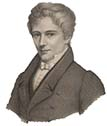
\includegraphics[width=0.13\textwidth]{abel.jpg}
 \end{enumerate}
 \vspace*{50pt}
  \end{definition}

  Most groups are not abelian. Example: in $GL_2()$, we have:

\[\begin{pmatrix}
1 & -1 \\ 0 & 2
\end{pmatrix}
\begin{pmatrix}
0 & 1 \\ 1 & 0
\end{pmatrix}
= 
\begin{pmatrix}
-1 & 1\\ 2 & 0
\end{pmatrix}\]

But 
\[
\begin{pmatrix}
0 & 1 \\ 1 & 0
\end{pmatrix}
\begin{pmatrix}
1 & -1 \\ 0 & 2
\end{pmatrix}
=
\begin{pmatrix}
0 & 2 \\ 1 & -1
\end{pmatrix}\]

So $\left(\begin{smallmatrix}
0 & 1\\ 1 & 0
\end{smallmatrix}\right)
$ and $\left(\begin{smallmatrix}
1 & -1\\ 0 & 2
\end{smallmatrix}\right)
$ do not commute, so $GL_2(\mathbb{R})$ is not abelian.\\


But many of the groups we have seen so far are abelian.\\

Examples: $(\Z,+), (F,+), (F\backslash\{0\},\times), GL_1(F), (\{1,-1,i,-i\},\times) $ are all abelian.\\

\begin{definition} Let $X$ be a set. A function $f : X \to X$ is a \emph{permutation}\index{Permutation} of $X$ if it is a bijection. (Injective + surjective). 	
\end{definition}\vspace*{10pt}

\begin{examples} \begin{enumerate}
 \item $X = \{1,2,3,4\}$. $f : 1 \mapsto 2, ~2 \mapsto 3,~ 3\mapsto 4,~ 4 \mapsto 1 $ is a permutation.
 \item $X = \Z, f: n \mapsto n+3$ is a permutation.
 \item $X = \Z$, $f: n \mapsto 3n$ is \emph{not} a permutation, (not surjective).
 \end{enumerate}
 \end{examples}\vspace*{10pt}
 
\noindent \textbf{Notation for permutations} (First attempt.)    \lecturemarker{14}{13/02} 
\\

Assume that $X = \{1,\dots,n\}$. Let $f: X \to X$ be a permutation. We can write $f$ as a matrix with two rows: \[
\begin{pmatrix}
1 & 2 & \dots & n\\ f(1) & f(2) & \dots & f(n)	
\end{pmatrix}\]

is called \emph{two-row rotation.}\\

Examples: if $f : 1 \mapsto 2, ~2 \mapsto 3,~ 3\mapsto 4,~ 4 \mapsto 1 $, we can write $f$ as $\left(\begin{smallmatrix}
1 & 2 & 3 & 4\\ 2 & 3 & 4 & 1	
\end{smallmatrix}\right)$. If $g$ is $\left(\begin{smallmatrix}
1 & 2 & 3 & 4\\ 3 & 1 & 2 & 4	
\end{smallmatrix}\right)$, then $g: 1 \mapsto 3,~2 \mapsto 1, 3\mapsto 2, 4\mapsto 4$.\\


Let $f$ and $g$ be permutations of a set $X$. We define the \emph{composition}\index{Composition}, $f \circ g$ by $f \circ g(x) = f(g(x))$ for all $x \in X$. For example, if $f$ and $g$ are as in the example above, we have $f \circ g(1) = 4, f\circ g(2) = 2, f\circ g(3) = 3, f \circ g(4) = 1$. So $f\circ g =
 \left(\begin{smallmatrix}
1 & 2 & 3 & 4\\ 4 & 2 & 3 & 1	
\end{smallmatrix}\right)$.\\


\begin{proposition} Let $X$ be any set. Let $S$ be the set of all permutations of $X$. Let $\circ$ be the composition operation as above. Then $(S,\circ)$ is a group, called the \emph{symmetric group}\index{Symmetric Group} on $X$, written Sym$(X)$.	
\end{proposition}


\begin{proof}
We first check that $\circ$ is a binary operation on $S$. Certainly if $f: X \to X$ and $g: X \to X$, then $f \circ g: X \to X$. The composition of two bijections is a bijection. So if $f,g  \in S$, then $f\circ g \in S$.\\

Now the group axioms:\begin{enumerate}
\item \textsc{Associativity:} If $x \in X$, and $f,g,h \in S$, then $(f \circ g) \circ h(x) = (f\circ g)(h(x)) = f(g(h(x))) = f(g \circ h(x)) = f \circ(g \circ h(x))$. Since they agree on all $x \in X$, we have $(f \circ g) \circ h = f \circ(g \circ h)).$
\item \textsc{Identity:} Let $e$ be the permutation defined by $e(x) = x$ for all $x \in X$. Then we have $e\circ f(x) = f(x) = f \circ e(x)$ for all $f\in S$. So $e\circ f = f \circ e = f$.
\item \textsc{Inverses:} Bijections have inverses.
\end{enumerate} \vspace*{-10pt}
\end{proof}

\noindent \textbf{Further notation:} We almost always write symmetric groups multiplicatively. So write $fg$ for $f\circ g$, and so on.\\
 When $X = \{1,\dots,n\}$, we write $S_n$ for the Sym$(X)$.\\
 
 
\begin{examples} $S_1$ = Sym$(\{1\}) = \{e\} = (	1,1)^T$.\\
 
 $S_2 = $ Sym$\{1,2\}$ = $\{e, \left(\begin{smallmatrix}
1 & 2 \\ 2 & 1	
\end{smallmatrix}\right)\}$\\

$S_3 = $ Sym$\{1,2,3\}$ = $\{e, \left(\begin{smallmatrix}
1 & 2 & 3 \\ 2 & 3 & 1	
\end{smallmatrix}\right),\left(\begin{smallmatrix}
1 & 2 & 3 \\ 3 & 1 & 2
\end{smallmatrix}\right),\left(\begin{smallmatrix}
1 & 2 & 3 \\ 2 & 1 & 3	
\end{smallmatrix}\right),\left(\begin{smallmatrix}
1 & 2 & 3 \\ 3 & 2 & 1
\end{smallmatrix}\right),
\left(\begin{smallmatrix}
1 & 2 & 3 \\ 1 & 3 & 2
\end{smallmatrix}\right)
\}$.

We have $|S_1| = 1, |S_2| = 2, |S_3| = 6$
\end{examples}\vspace*{10pt}

\begin{proposition} The group $S_n$ has order $n!$	
\end{proposition}

\begin{proof}
	By induction. Inductive hypothesis. if $X$ and $Y$ are the two set of size $n$, then the number of bijections form $X$ to $Y$ is $n!$. (This gives us the result by taking $Y=X$.)\\
	
	Base case $n=1$ is obvious.\\
	Inductive step: Suppose the result is true for $n$:\\
	
	Let $|X| = |Y| = n+1$. Take $x \in X$, $y \in Y$. The number of bijections $f: X \to Y$ such that $f(x) = y$ is equal to the number of bijections $X\backslash\{x\} \to Y\backslash\{y\}$, which is $n!$ by the inductive hypothesis. So the total number of bijections $X \to Y$ is $(n+1)n! =  (n+1)!$.
\end{proof}


\noindent \textbf{The Group Table.} Let $G$ be a finite group. We can record the multiplication (binary operation) in $G$ in a table called the \emph{Group Table} or \emph{Cayley Table}\index{Group Table} of $G$. If $G =\{a,b,c,\dots\}$, write:
 \[
    \begin{tabular}{>{$}l<{$}|*{4}{>{$}l<{$}}}
    ~  & a   & b   & c & \dots  \\
    \hline\vrule height 12pt width 0pt
    a   & aa  & ab    & ac & ~  \\
    b   & ba   & bb & bc  & \dots   \\
    c & ca & cb    & cc  &~   \\
    \vdots & ~ & \vdots & ~ & ~
    \end{tabular} 
\]

\begin{example} Let $G = S_3$\\

 Write $a = \left(\begin{smallmatrix}
1 & 2 & 3 \\ 2 & 3 & 1	
\end{smallmatrix}\right).$ Then $a^2 = \left(\begin{smallmatrix}
1 & 2 & 3 \\ 3 & 1 & 2
\end{smallmatrix}\right),$ and $a^3 = e$.\\

Write $b = \left(\begin{smallmatrix}
1 & 2 & 3 \\ 1 & 3 & 2	
\end{smallmatrix}\right).$ Then $b^2= \left(\begin{smallmatrix}
1 & 2 & 3 \\ 2 & 1 & 3
\end{smallmatrix}\right),~ a^2b
\left(\begin{smallmatrix}
1 & 2 & 3 \\ 3 & 1 & 2
\end{smallmatrix}\right)$.\\

So $S_3 = \{e, a, a^2, b, ab, a^2b\}$. To work out the group table, it is helpful to check: $b^2 = e, ba = a^2b, ba^2 = ab$. Now it is easy to write down:

 \[
    \begin{tabular}{>{$}l<{$}|*{6}{>{$}l<{$}}}
    ~  & e   & a   & a^2 & b & ab & a^2b  \\
    \hline\vrule height 12pt width 0pt
    e  & e  & a & a^2    & b & ab & a^2b \\
    a   & a & a^2 & e & ab & a^2b & b\\
    a^2 & a^2 & e & a & a^2b  & b  & ab \\
    b & b & a^2b & ab & e & a^2 & a\\
    ab & ab &  b & a^2b & a & e & a^2\\
    a^2b & a^2b & ab & b & a^2 & a & e
    \end{tabular} 
\]

Notice that every element of the group appears exactly once in each row and each column. (This follows from left and right cancellation laws.)
\end{example}


\subsektion{Subgroups}\vsp


\begin{definition} Let $(G,*)$ be a group. A \emph{subgroup}\index{Subgroup} of $G$ is a subset of $G$ which is itself a group under the operation $*$.	
\end{definition}\vspace*{10pt}


\begin{examples}\begin{enumerate}
 \item[(i)] $(\Z,+)$ is a subgroup of $(\Q,+)$. Both are subgroups of $(\mathbb{R},+)$. All are subgroups of $(\C,+)$. But $(\mathbb{N},+)$
 is not a subgroup of any - it has no inverses.
 \item[(ii)] $(\mathbb{R} \backslash\{0\},\times)$ is not a subgroup of $(\mathbb{R},+)$. The group operation is different.
 \item[(iii)] $\{e\}$ is a subgroup of any group (where $e$ is the identity element). The \emph{trivial} subgroup.
 \item[(iv)] Every group is a subgroup of itself.
  \end{enumerate}
  \end{examples}

\emph{Recall:} \lecturemarker{15}{17/02} 
a subgroup of a group $G$ is a subset of $G$ which is a group under the same operation as $G$.\\

\begin{proposition} (Subgroup Criteria) Let $G$ be a group. We write $G$ multiplicatively. Let $H \subseteq G$ be a subset. Then $H$ is a subgroup if and only if the following conditions hold:\begin{enumerate}
\item $e \in H$, where $e$ is the identity of $G$.
\item If $a,b \in H$, then $ab \in H$, for all $a,b \in G$.
\item If $a \in H$, then $a^{-1} \in H$, where $a^{-1}$ is the inverse of $a$ in $G$.	
\end{enumerate}
\end{proposition}

\begin{proof}
\textbf{``if''}. Condition (2) says that the binary operation on $G$ restricts to a binary operation on $H$. Since the operation is associative on $G$, it is also associative on $H$. Condition (1) gives us an identity, and Condition (3) gives inverses. So if (1),(2),(3) hold then $H$ is a subgroup.\\

\textbf{``only if''}. Certainly (2) must hold if $H$ is a subgroup, since we need the binary operation on $G$ to restrict to a binary operation on $H$. If $H$ is a subgroup, then $H$ has an identity, $e_H$. Write $e_G$ for the identity of $G$. Then $e_Ge_H = e_H$, and also $e_He_H = e_H$. Now $e_G = e_H$, by right cancellation. So $e_G \in H$, and so (1) holds.\\

Let $a \in H$. Let $b$ be the inverse of $a$ in $G$, and let $c$ be the inverse of $a$ in $H$. $ab = e_G = e_H = ac$. So $b=c$ by left cancellation. So $b \in H$, and so (3) holds.
\end{proof}\vspace*{10pt}

\begin{example} Let $G = GL_2()$. For $n \in \Z$, define $u_n = \left(\begin{smallmatrix}
1 & n \\ 0 & 1	
\end{smallmatrix}\right)
$, so $u_n \in G$, for all $n \in \Z$. Define $U = \{u_n ~:~ n \in \Z\}$. Then $U$ is a subgroup of $G$. Check the subgroup criteria: \begin{enumerate}
 \item $e_G = I = u_0 \in U$
 \item $u_mu_n = \left(\begin{smallmatrix}
1 & m \\ 0 & 1	
\end{smallmatrix}\right)\left(\begin{smallmatrix}
1 & n \\ 0 & 1	
\end{smallmatrix}\right) = 
\left(\begin{smallmatrix}
1 & m+n \\ 0 & 1	
\end{smallmatrix}\right) = u_{m+n} \in U$	
\item From (1) and (2), we see that $u_m^{-1} = u_{-m}$, so $u_{m}^{-1} \in U$. So $U$ is a subgroup.
 \end{enumerate} 
 \end{example}
 
\noindent \textbf{Notation:} If $H$ is a subgroup of $G$, we write $H \leq G$. (We can write $H < G$ if $H \neq G$).\\

\noindent \textbf{Powers in groups:} Let $G$ be a a group written multiplicatively. Let $g \in G$. We can write $g^1 = g, ~ g^2 = gg,~ g^3 = ggg$, and so on. We also write $g^{0} = e$, and $g^{-n} = (g^{-1})^n$. So now $g^n$ is defined for all $n \in \Z$.\\

\begin{proposition}\begin{itemize}
 \item[(a)] $(g^n)^{-1} = g^{-n}$.
 \item[(b)] $g^mg^n = g^{m+n}$.
 \item[(c)] $(g^m)^n = g^{mn}$.	
 \end{itemize}
 \end{proposition}
 
 \emph{Proof omitted.}
 
\begin{warning} It is not generally true that $a^nb^n = (ab)^n$. (Though true for Abelian Group)	
\end{warning}

\subsektion{Cyclic Subgroups} 
\begin{proposition} Let $G$ be a group, and let $g \in G$. Define $\langle g\rangle  = \{g^n : n \in \Z\}$. Then $\langle g\rangle $  is a subgroup of $G$.	
\end{proposition}

 \begin{proof}
 	Check subgroup criteria: \begin{enumerate}
 \item $g^{0} = e$
 \item $g^mg^n = g^{m+n}$
 \item $(g^n)^{-1} = g^{-n}$ \qedhere 
 \end{enumerate}\end{proof}\vspace*{10pt}
 

\begin{definition} The subgroup $\langle g \rangle$ is the \emph{cyclic subgroup}\index{Cyclic Subgroup} generated by $g$.
	
\end{definition}\vspace*{10pt}

\begin{examples} \begin{enumerate}
 \item $U = \{u_n = \left(\begin{smallmatrix}
1 & n \\ 0 & 1	
\end{smallmatrix}\right) ~:~ n \in \Z
\}$	is $\langle u_1 \rangle $. (Easy induction to show that $\left(\begin{smallmatrix}
1 & 1 \\ 0 & 1	
\end{smallmatrix}\right)^n = \left(\begin{smallmatrix}
1 & n \\ 0 & 1	
\end{smallmatrix}\right)$ for all $n \in Z$)
\item In $(\Z,+),$ what is $\langle 3 \rangle $?\\
Note that we write this group additively, write $ng$ instead of $g^n$. So $\langle 3 \rangle = \{n.3 ~:~ n \in \Z\}$. So $\langle 3 \rangle$ contains precisely all multiples of 3.
\item $G = S_3$. What are the cyclic subgroups? From the group table we can easily calculate:\\\vspace{5pt}
$\langle e \rangle = \{e\}$\\ \vspace{5pt}
$\langle a \rangle = \{e,a,a^2\}$, since $a^3 = e$.\\\vspace{5pt}
$\langle a^2 \rangle = \{e,a,a^2\}$\\\vspace{5pt}
$\langle b\rangle = \{e,b\}$ since $b^2 = e$\\\vspace{5pt}
$\langle ab \rangle = \{e,ab\}$, since $(ab)^2 = e$\\\vspace{5pt}
$\langle a^2b \rangle = \{e,a^2b\}$, since $(a^2b)^2 = e$\\
 \end{enumerate}
 \end{examples}\vspace*{5pt}
 
%\textit{Recall:} %$\langle g \rangle = \{g^n : n \in \Z\}$

\begin{definition}  \lecturemarker{16}{18 /02} 
A group is \emph{cyclic}\index{Cyclic Group} if $G = \langle g \rangle $ for some $g \in G$. In this case $g$ is a \emph{generator}\index{Generator} for $G$.
	
\end{definition}

\begin{examples}\begin{enumerate}
\item[(i)] $(\Z,+)$	is cyclic, since $\Z = \langle 1 \rangle$. Another generator is $-1$. There are no other generators.
\item[(ii)] $\{1,-1,i,-i\}$ is cyclic, since it is equal to $\langle i \rangle $, and $\langle -i \rangle$. So $i$ and $-i$ are generators. 1 and $-1$ are not.
\item[(iii)] Let $\Omega_n = \{$ complex $n$th roots of unity $\}$, under complex multiplication. Let $w = e^{2\pi i/n}$. Then $\langle w \rangle = \{e^{2\pi i k/n} : k \in \Z\} = \Omega_n$. So $\Omega_n$ is a a group - a cyclic subgroup of $\C$.

Since $|\Omega_n| = n$, it follows that there exists a group of order $n$ for $n \in \mathbb{N}$.

\item[(iv)] $S_3$ is \emph{not} cyclic. We have calculated all of its cyclic subgroups (Example 76, 3), and none of them were equal to $S_3$.
 \end{enumerate}
 \end{examples}
 
 \subsektion{The Order of a Group Element}\vsp
 
\begin{definition} Let $G$ be a group, and $g \in G$. The \emph{order}\index{Order of Element} of $g$ is the least positive integer $k$, such that $g^k = e$, if such an integer exists. Otherwise $g$ has infinite order. Write ord$(g)$ or o$(g)$ for the order of $g$. Write ord$(g) = \infty$ if $g$ has infinite order.	
\end{definition}\vspace*{10pt}

\begin{examples}\begin{enumerate}
 \item[(i)] In any group $G$, the identity $e$ has order 1. No other element has order 1. (If $g^1 = e$ then $g = e$.)
 
 \item[(ii)] Let $G = S_3$ Let $a  = \left(\begin{smallmatrix}
1 & 2 & 3 \\ 2 & 3 & 1	
\end{smallmatrix}\right)$. Then $a^1 \neq e$, $a^2 = \left(\begin{smallmatrix}
1 & 2 & 3 \\ 3 & 1 & 2 	
\end{smallmatrix}\right) \neq e$. But $a^3 = e$. So ord $(a)$ = 3.

 Let $b = \left(\begin{smallmatrix}
1 & 2 & 3 \\ 1 & 3 & 2	
\end{smallmatrix}\right).$ Then $b \neq e$, but $b^2 = e$. So ord$(b)$ = 2. Can also check that ord$(a^2)$ = 3, ord$(ab)$ = 2, ord$(a^2b)$ = 2.


\item[(iii)] Let $G = (\Z,+)$. We know that ord$(0)$ = 1. Suppose $n \neq 0$. Then since $\underbrace{n + n + \dots n}_{k} = kn \neq 0$ for any positive integer $k$. We must have ord $(n)$ = $\infty$.
\item[(iv)] $G = GL_2(\C)$. Let $A = \left(\begin{smallmatrix}
i & 0 \\ 0 & e^{2 \pi i/3} 	
\end{smallmatrix}\right)$. \emph{What is the order of $A$?}

We see that for $k \in \Z$ we have $A^k = \left(\begin{smallmatrix}
i^k & 0 \\ 0 & e^{2\pi ik/n}	
\end{smallmatrix}\right)
$, which is equal to $\left(\begin{smallmatrix}
1 & 0 \\ 0 & 1	
\end{smallmatrix}\right)$ if and only if $i^k = 1$ and $e^{2 \pi ik/n} = 1$.

 Now $i^k = 1$ if and only if $4 ~|~ k$, and $e^{2\pi ik/n} = 1$ if and only if $3 ~|~ k$. So $A^k = I$ if and only if $12 ~|~ k$. Since the smallest positive integer divisible by 12 is 12, we have ord($A$) = 12.
 \end{enumerate}
 \end{examples}
 
\begin{proposition} If $G$ is a group and $g \in G$, then $|\langle g \rangle| = $ ord $(g)$. ($\langle g \rangle$ is infinite $\iff$ ord $(g) = \infty$).	
\end{proposition}

 
 \begin{proof}
 Suppose first that ord$(g) = \infty$. So $g^k \neq e$ for any $k \in \mathbb{N}$. We claim that if $m \neq n \in \Z$, then $g^m \neq g^n$. Suppose w.l.o.g. that $n > m$. Let $k = n-m$. Then $k \in \mathbb{N}$. Now $g^n = g^{m+k} = g^mg^k$. If $g^m = g^n$, then $g^m = g^mg^k$, and so $g^k = e$ by left cancellation. But this is a contradiction, and this proves the claim.\\
 Now we have $g^0,g^1,g^2,g^3,\dots$ are all distinct elements of $\langle g \rangle$, and so $\langle g \rangle$ is infinite.\\
 
 Now suppose that ord$(g) = k \in \mathbb{N}$. I claim that $\langle g \rangle = \{g^0,g^1,\dots,g^{k-1}\}$, and that the elements $g^0,\dots,g^{k-1}$, are distinct. (So $|\langle g \rangle| = k$). We use the fact that $n \in \Z$ can be written as $pk + q$, where  $p,q \in \Z$ and $0 \leq q < k$. So $g^n = g^{pk+q} = (g^k)^pg^q = e^pg^q = g^q$. But $g^q$ is one of the elements $g^0,\dots,g^{k-1}$, and so $\langle g \rangle = \{g^0,\dots,g^{k-1}\}$.\\
 
  Suppose $g^i = g^j$, where $0 \leq i < j \leq k-1$. Let $l = j-i.$ Then $g^i = g^j = g^{i + l}$, and so $g^l = e$ by left cancellation. But $l$ is a positive integer less than $k$, so this contradicts the assumption that ord$(g)$ = $k$. This proves the claim.
 \end{proof}


We have seen Proposition 81 illustrated in several examples already.\\

\begin{examples} \begin{enumerate}
 \item[(i)] Comparing the list of cyclic subgroups of $S_3$ with the list of the orders of elements, we saw that ord$(g) = |\langle g \rangle|$ in each case.
 \item[(ii)] In the case $G = (\Z,+)$, we saw that $\langle 3 \rangle = 3\Z = \{3k : k \in \Z\}$. So $|\langle 3 \rangle| = \infty$, and we have also seen that ord$(3) = \infty$.
 \item[(iii)] If $w = e^{2\pi i/n}$, then clearly ord$(w) = n$. And $\langle w \rangle = \Omega_n$ has order $n$ too.	
 \end{enumerate}
\end{examples}\vspace*{10pt}

\subsektion{Cycles}
 
Let \lecturemarker{17}{20/02} 
 $f = \left(\begin{smallmatrix}
1 & 2 & 3 & 4 & 5 & 6 & 7 & 8 \\
4 & 5 & 6 & 3 & 2 & 7 & 1 & 8	
\end{smallmatrix}\right)$. Looking at the successive images of 1 under the permutation $f$, we get back to 1 again after 5 steps via 4,3,6,7.


\begin{center}   
 \begin{tikzpicture}
 $f$~~
\node (P0) at (90:1.4cm) {$1$};
\node (P1) at (90+72:1.4cm) {$7$} ;
\node (P2) at (90+2*72:1.4cm) {$6$};
\node (P3) at (90+3*72:1.4cm) {$3$};
\node (P4) at (90+4*72:1.4cm) {$4$};
\draw
(P0) edge[<-|,>=angle 90] node[left] {} (P1)
(P1) edge[<-|,>=angle 90] node[left] {} (P2)
(P2) edge[<-|,>=angle 90] node[above] {} (P3)
(P4) edge[|->,>=angle 90] node[right] {} (P3)
(P0) edge[|->,>=angle 90] node[right] {} (P4);
\end{tikzpicture}
\end{center}


We say that 1,4,3,6,7 forms a 5-cycle of $f$. Write $(1 ~4~ 3 ~6~ 7)$ for this cycle.\\

Similarly:\begin{tikzcd}
2\arrow[mapsto,bend left]{r} \arrow[mapsfrom,bend right]{r}{f}&5
\end{tikzcd} is a 2-cycle, written $(2~5)$.\\

 Finally 8 is a fixed point or 1-cycle of $f$. We can write $(8)$ if we like $-$ but usually we do not write out 1-cycles.\\
 
 
 We can think of cycles as permutations in their own right. Take everything outside the cycle to be fixed.\\
 
  So $(1~4~3~6~7)$ is the permutation: $\left(\begin{smallmatrix}
1 & 2 & 3 & 4 & 5 & 6 & 7 & 8\\
4 & 2 & 6 & 3 & 5 & 7 & 1 & 8 	
\end{smallmatrix}\right)$.\\

 And $(2~5)$ is the permutation: $\left(\begin{smallmatrix}
1 & 2 & 3 & 4 & 5 & 6 & 7 & 8\\
1 & 5 & 3 & 4 & 2 & 6 & 7 & 8 	
\end{smallmatrix}\right)$. \\

And $(8)$ represents the identity permutation.\\


Notice that $f =  (1~4~3~6~7)(2~5)$ (where the cycles are multiplied by composition, as elements of $S_8)$. So we have factorised $f$ into cycles. These cycles have no common points $-$ they are disjoint. This is the \emph{disjoint cycle notation}\index{Disjoint Cycles} for $f$.\\


\begin{method}To calculate the disjoint cycle notation for a permutation $f \in S_n$.

Step 1. Pick the least element $i \in \{1,\dots,n\}$ which  we haven't used yet. (Initially, we choose $i=1$.) Open a new cycle with $i$. 

Step 2. Continue the cycle with successive images of $i$ under $f$ until we get back to $i$ again. Then close the cycle.

Step 3. If all $i \in \{1,\dots,n\}$ have appeared, then stop. Otherwise go back to Step 1.

\end{method}\vspace*{10pt}

\begin{examples}$f = \begin{pmatrix}
1 & 2 & 3 & 4 & 5 & 6 & 7 & 8 & 9 & 10\\
3 & 6 & 1 & 7 & 5 & 8 & 2 & 4 & 10 & 9	
\end{pmatrix}$. \\

Open a cycle with 1. Continue the cycle with $f(1) = 3$. Since $f(3)$ is 1 again, close the cycle. $(1~3)$. Now open a new cycle with 2. Continue it with 6,8,4,7. Since $f(7) = 2$, we then close the cycle. $(2~6~8~4~7)$. Start a cycle with 5. But 5 is a fixed-point of $f$, so close the cycle immediately. $(5)$. Finally, start a cycle with 9. Continue it with $f(9) = 10$. But $f(10) = 9$, so close the cycle. $(9~10)$.

Now all points have appeared, so we stop. So the disjoint cycle notation for $f$ is $f = (1~3)(2~6~8~4~7)(5)(9~10)$. We usually omit 1-cycles. So $f = (1~3)(2~6~8~4~7)(9~10)$.
\end{examples}\vspace*{5pt}

\begin{proposition} Method 83 always works. Every permutation in $S_n$ can be written as a product of disjoint cycles.	
\end{proposition}


\begin{proof}
	First we show that whenever we open a new cycle at Step 1, we are able to close it at Step 2. (We always get back to the starting point eventually.)
	
	Suppose that $x$ is the starting point. Since $n$ is finite, the points $x, f(x), f^2(x),\dots$ cannot be all distinct. So there must exist some least $k$ such that $f^k(x) = f^j(x)$, for some $j < k$. Suppose that $j \neq 0$. Then $f^{-1}f^k(x) = f^{-1}f^j(x),$ and so $f^{k-1}(x) = f^{j-1}(x)$.
	
	 But this contradicts the assumption that $k$ was the \emph{least} to give a repeat. So by contradiction, we must have $j = 0$. So $f^k(x) = f^0(x) = x$. So the first repeated term in the cycle is $x$ itself, and we close the cycle at that point.
	 
	 Next we check that the cycles arising from Method 83. are disjoint. Let $c$ and $d$ be two cycles. Suppose that $c$ starts with $x$ and $d$ starts with $y$. Suppose that $c$ was constructed first. Then $y$ cannot be in the cycle $c$ (since otherwise we would not have used it to start a new cycle.)
	 
	 Suppose $z$ is in both $c$ and $d$. So $z = f^i(x) = f^j(y)$ for some $i,j$. But now $f^{i-j}(x) = y$ This implies that $y$ is in the cycle $c$, which is a contradiction. Hence $c$ and $d$ are disjoint.
\end{proof}\vspace*{5pt}


\noindent \textbf{Multiplication.} To multiply permutations given in disjoint cycle notation, recall that $fg = f \circ g,$ so $fg(x) = f(g(x))$. Use Method 83 to get the disjoint cycle notation of $fg$. 

\textit{Example:} $f = (1~3~5)(2~4~6)$, $g = (1~2~3~4)(5~6) \in S_6$. Calculate $fg: 1 \mapsto 4 \mapsto 3 \mapsto 6 \mapsto 1\quad $ $2\mapsto 5 \mapsto 2$. Hence $fg = (1~4~3~6)(2~5)$.\\
 
 
 \noindent \textbf{Inverses.} These are very easy~ Just write the cycles backwards.
 
E.g. If $f = (1~3~5)(2~4~6)$, then $f^{-1} = (5~3~1)(6~4~2) = (1~5~3)(2~6~4)$.\\
  
 \noindent \textbf{Non-uniqueness.} \begin{enumerate}
 \item[i.] Order of the cycles doesn't matter.	
 \item[ii.] The choice of starting point in each cycle doesn't matter.
 \item[iii.] We can include or exclude 1-cycles.
 \end{enumerate}\vspace*{5pt}
 
\begin{example}\lecturemarker{18}{24/02} 
 In disjoint cycle notation, the group table for $S_3$ from Example 68 becomes:


 \[
    \begin{tabular}{>{$}l<{$}|*{6}{>{$}l<{$}}}
    ~  & e   & (123)   & (132) & (23) & (12) & (13)  \\
    \hline\vrule height 12pt width 0pt
    e  & e   & (123)   & (132) & (23) & (12) & (13) \\
    (123)   & (123) & (132) & e & (12) & (13)& (23)\\
    (132) & (132) & e & (123) & (13) & (23) & (12) \\
    (23) & (23) & (13) & (12) & e & (132) & (123)\\
    (12) & (12) &  (23) & (13) & (123) & e & (132)\\
    (13) & (132) & (12) & (23) & (132)& (123) & e
    \end{tabular} 
\]
\end{example}
\vspace*{10pt}

\begin{remark} Disjoint cycles commmute. (If cycles $c_1$ and $c_2$ have no points in common, then $c_1c_2 = c_2c_1$). Example: $(12)(345) = (345)(12)$.\\

 Cycles which are not disjoint don't usually commute. Example: $(12)(13) = (132)$. $(13)(12) = (123)$.
 \end{remark}\vspace*{10pt}
 

\begin{definition} The \emph{cycle shape}\index{Cycle Shape} of a permutation is the sequence of cycle lengths in descending order of size when the permutation is written in disjoint cycle notation. We include $1-$cycles.	
\end{definition}\vspace*{10pt}

Example: $f = (12)(3)(456)(7)(89) \in S_9$ then $f$ has cycle shape $(3,2,2,1,1)$. We abbreviate this to $(3,2^2,1^2).$ The identity of $S_9$ has cycle shape $(1,1,1,1,1,1,1,1,1),$ or  $(1^9)$.\\


\begin{examples}What are the cycle shapes in $S_4$, and how many elements are there of each shape?\\

Cycle shapes are given by weakly decreasing sequences of positive integers adding up to 4. There are $(4)$, $(3,1)$, $(2^2)$, $(2,1^2)$ and $(1^4)$. (These are the \emph{partitions} of the integer 4). How many of each type? \begin{itemize}
 \item[$(4)$:] May start the cycle at 1. There are 3 choices for $f(1)$. Then there are 2 choices for $f^2(1)$. This determines the cycle. So 6 possible 4-cycles. (These are $(1234),~(1243),~(1324),~(1342),~(1423),(1432)$.)
 \item[$(3,1)$:] There are 4 choices for the fixed-point (or 1-cycle).  Once the fixed point is chosen, there are 2 choices for the 3-cycle. So there are 8 possible permutations with this shape.
 \item[$(2^2)$:] 1 is in a 2-cycle, and there are 3 choices for the other point in that cycle. This determines the permutation. So there are only 3 permutations with this shape. These are $(12)(34),~(13)(24),~(14)(23)$.
 \item[$(2,1^2)$:] There are $\left(\begin{smallmatrix}
4 \\ 2	
\end{smallmatrix}\right)$ ways of choosing the two fixed points. This determines the permutations. So there are 6 permutations.
\item[$(1^4)$:] Only the identity has this shape. 
 \end{itemize}
 
 Check: we have $6 + 8 + 3 + 6 + 1 = 24 = |S_4|$.
\end{examples}


 \subsektion{Order of a Permutation}
 
\begin{proposition} Let $G$ be a group, and let $g \in G$. Suppose ord$(g) = d$. Then for all $k\in \Z$, we have $g^k = e \iff d~|~k $.	
\end{proposition}

 
 \begin{proof}
 By Euclid's Lemma, we can write $k = xd + y,$ where $x,y \in \Z$ and $0 \leq y < d$. Now $g^k = g^{xd + y} = (g^d)^xg^y = e^xg^y = g^y$. But $y < d$, and so we have $g^y = e \iff y =0 \iff d~|~k$.
 \end{proof}
 
\begin{proposition}Let $G$ be a group, and let $a,b\in G$ be elements such that $ab = ba$. Then: \begin{enumerate}
 \item $a^{-1}b = ba^{-1}$
 \item $a^ib^j = b^ja^i$, for $i,j \in \Z$.
 \item $(ab)^k = a^kb^k$, for $k \in \Z.$	
 \end{enumerate}
 \end{proposition}
 
 \begin{proof}~\\[-.1cm]
 
 (i). We have $ab = ba.$ So $a^{-1}(ab)a^{-1} = a^{-1}(ba)a^{-1}$. Hence $ba^{-1} =  a^{-1}b$.
 
 (ii). If $j < 0$, then replace $b$ with $b^{-1}$. We know $ab^{-1} = b^{-1}a$ by 1. In this way, we may assume $j \geq 0$. Now by induction on $j$. [left as exercise.]
 
 (iii). If $k < 0$, then write $d = a^{-1},~c = b^{-1}$. Then $(ab)^{-1} = cd$, and so $(ab)^k = (cd)^{-k}$. In this way we may assume $k \geq 0$. Now work by induction on $k$. [left as exercise.]
 \end{proof}\vspace*{5pt}

 
 
\begin{proposition} Let $f$ be a permutation with cycle shape $(r_1,r_2,\dots,r_k)$. Then ord$(f) =$ lcm$(r_1,r_2,\dots,r_k)$.	
\end{proposition}


 \begin{proof} 

Write  \lecturemarker{19}{25/02} $f = c_1c_2\dots c_k$, where $c_i$ has length $r_i$ for all $i$, and the cycles $c_i$ are disjoint from one another.\\

Recall \textit{Remark 87}: disjoint cycles commute. So $c_ic_j = c_jc_i$, for all $i,j$. Let $t \in \Z$. \textbf{Claim:} $f^t = c_1^tc_2^t\dots c_k^t$. 
\begin{proof}[Proof of Claim] First observe that $f = c_1,\dots,c_{k-1}c_k = c_kc_1,\dots,c_{k-1}$, since $c_k$ commutes with all of the other cycles. So $c_k$ commutes with $c_1\dots c_{k-1}$. So by Prop 91.3, we have $f^t = ((c_1\dots c_{k-1})c_k)^t =(c_1\dots c_{k-1})^t  c_k^t $. Now an easy induction on $k$ gives that $f^t = c_1^tc_2^t\dots c_k^t$, as required.
\end{proof}

Continuing the proof of Prop 92, we see that $f^t = e \iff c_i^t = e$, for all $i$. But $c_i^t = e$ if and only if $r_i ~|~ t$. So $f^t = e \iff r_i ~|~ t$, for all $i \iff t$ is divisible by lcm$(r_1,r_2,\dots,r_k)$.\\

So ord$(f)$ is the last positive integer divisible by lcm$(r_1,\dots,r_k)$, which is lcm$(r_1,\dots,r_k)$ itself.
 \end{proof}\vspace*{10pt}
 
\begin{examples} \begin{enumerate}
 \item[(i)] ord$((12)(3456))$ = lcm$(2,4) = 4.$
 \item[(ii)] ord$(13)(3456)) \neq 4 -$ the cycles are not disjoint. We calculate $(13)(3456) = (13456)$, which has order 5.
 \item[(iii)] Clearly 1-cycles never affect the order of a permutation.
 \item[(iv)] Suppose we have a pack of 8 cards. We shuffle them by cutting the pack into 2 equal parts, and then interleaving the parts. \vspace*{-5pt}
 
 We get the permutation $\left(\begin{smallmatrix}
	1 & 2 & 3 & 4 & 5 & 6 & 7 & 8 \\ 1 & 5 & 2 & 6 & 3 & 7  & 4 & 8
\end{smallmatrix}\right).$ In disjoint cycle form, this is $(253)(467)$, which has order 3. So if we repeat our shuffle three times, the pack is back in its original order.
\end{enumerate}
\end{examples}\vspace*{10pt}

\textit{Exercise: How many shuffles do you need for a full pack of 52 cards to be shuffled back to its original order?}

 
 \subsektion{Lagrange's Theorem}\vsp 
 
 
\begin{theorem}[Lagrange's Theorem]\index{Lagrange's Theorem|idxbf}  Let $G$ be a finite group. Let $H$ be a subgroup of $G$. Then $|H|$ divides $|G|$.	
\end{theorem}\vspace*{10pt}

 
\begin{examples}\begin{enumerate}
 \item $|S_3| = 6$. We have seen that the cyclic subgroups of $S_3$ have orders $1,2,3$. There are no other subgroups, except $S_3$ itself.
 \item $G = \{1,-1,i,-i\}$, order 4. The subgroups of $G$ are $\{1\},\{1,-1\}$, and $G$, with orders $ 1,2,4.$
 \item Let $C_n = \langle w \rangle \leq \C \backslash\{0\}$, where $w = e^{2\pi i/n}$. If $d$ divides $n$, then $w^{n/d} = e^{2\pi i/d}$, which has order $d$. So $\langle w^{n/d} \rangle$ is a subgroup of $C_n$ with order $d$. In fact all of the subgroups of $C_n$ have this form, for some $d$.
 \end{enumerate}
 \end{examples}\vspace*{10pt}

\noindent \textit{Remark.} Although it is true for the elementary groups above, it is not true in general that a group $G$ has a subgroup of order $d$ for every divisor.\\
 Example: $S_5$ has order 120, but has no subgroup of order $15,30,40$.\\
 
 
\begin{corollary} (to Lagrange's Theorem) If $G$ is a finite group, and $g \in G$, then ord$(g)$ divides $G$.	
\end{corollary}


\begin{proof}
ord$(g) = |\langle g \rangle|,$ and this divides $G$ by Lagrange's Theorem.	
\end{proof}\vspace*{5pt}

\begin{corollary}Suppose $|G| = n$. Then $g^n = e$, for all $g \in G.$	
\end{corollary}

\begin{proof}
We know ord$(g) ~|~ n$ by Corollary 96. So $g^n = e$ by Prop 90.
\end{proof}\vspace*{5pt}

\begin{corollary} If $|G|$ is a prime number, then $G$ is cyclic.	
\end{corollary}

\begin{proof}
Let $g \in G$ be such that $g \neq e$. Then ord$(g)\neq 1$, but ord$(g) ~|~ |G|$. So ord$(g) = |G|$ (Since $|G|$ is prime.)	Hence $\langle g \rangle = G$, and so $G$ is cyclic.
\end{proof}\vspace*{5pt}


\textbf{Some ideas for the proof of Lagrange's Theorem.}

$G$ is a finite group. $H \leq G$ is a subgroup. We shall divide the elements of $G$ into disjoint subsets, so that every element is in exactly one subset, and each subset has the same size as $H$. Now if there are $k$ subsets, then $|G| = k|H|$, and we are finished.\\

\textit{What are these subsets?} One of these will be $H$ itself. Now if $x \in G\backslash H$, we need a subset including $x$. We take $Hx = \{hx : h \in H\}$. Now if $y \in G \backslash(H \cup Hx)$, then we take $Hy$, and keep on going until we have used up all the elements of $G$.\\

\begin{definition}  \lecturemarker{20}{27/02} 
Let $G$ be a group, and let $H \leq G$. Let $x \in G$. The \emph{right coset}\index{Cosets} $Hx$ is the set $\{hx : h \in H\}$. [The \emph{left coset} $xH$ is the set $\{xh : h \in H\}$.\end{definition}\vspace*{5pt}

\begin{claim} $|Hx| = |H|$, for all $x \in G$. 	
\end{claim}

\begin{proof}

It is enough to show that $h_1x \neq h_2x$, if $h_1 \neq h_2$. But this is true by right cancellation, since $h_1x = h_2x \implies h_1 = h_2$.
\end{proof}\vspace*{5pt}


\begin{claim} Let $x,y \in G$. Then either $Hx = Hy$, or else $Hx \cap Hy = \emptyset$. (Two right cosets of $H$ are equal or disjoint.)	
\end{claim}

\begin{proof}
	Suppose that $Hx$ and $Hy$ are not disjoint. So there exists $z \in Hx \cap Hy$. So there exists $h_1,h_2 \in H$ such that $z = h_1x = h_2y$. Now $y = h_2^{-1}h_1x$, and so $y \in Hx$. Now any $hy$ in $Hy$ is equal to $hh_2^{-1}h_1x$, which is in $Hx$. So $Hy \subseteq Hx$. By a similar argument, $Hx \subseteq Hy$ and so $Hx = Hy$.
\end{proof}\vspace*{5pt}

\begin{claim} $x \in Hx$ for all $x \in G$.	
\end{claim}

\begin{proof}
$e \in H$, and so $x = ex \in Hx$. 	
\end{proof}

\begin{proof}[\textbf{Proof of Lagrange's Theorem}]~\\[-.2cm]

	Consider the set $S = \{Hx : x \in G\}$, a set of cosets. \begin{enumerate}
 \item[(i)] Every $x \in G$ is in one member of $S$. (By Claim 102.)
 \item[(ii)] Every $x \in G$ is in no more than one member of $S$. (By Claim 101.)
 
 It follows that $\displaystyle{ |G| = \sum_{X \in S} |X|}$
 \item[(iii)] Every member of $S$ has size $|H|$. (By Claim 100.)

 \end{enumerate}
 Hence $|G| = k|H|,$ where $|S| = k$. So $|H|$ divides $|G|$ as required.
\end{proof}

\begin{remarks} (Further Properties of cosets) \begin{enumerate}
 \item  $H = Hx \iff x \in H$.\begin{proof}
Notice that $H = He$, so is a coset. If $x \in H$, then certainly $H \cap Hx \neq \emptyset$, so $H = Hx$, by Claim 101.	If $x \neq H$, then $H \neq Hx$, since $x \in Hx$.
\end{proof}
\item If $y \in Hx$, then $Hx = Hy$. \begin{proof}
 We have $y \in Hx \cap Hy$, and so $Hx \cap Hy \neq \emptyset$. So $Hx = Hy$, by Claim 101.	
 \end{proof}
 
 \item If $x \not\in H$, then $Hx$ is \emph{not} a subgroup of $G$. \begin{proof}
 	$H \cap Hx = \emptyset$, by (1). Hence $e \not\in Hx$. 
 \end{proof}

\item $Hx = Hy$ if and only if $xy^{-1} \in H$.\begin{proof}
$Hx = Hy$ if and only if $x \in Hy$, and this occurs if and only if $x = hy$ for some $h \in H$. But this is equivalent to $xy^{-1} = h$.	
\end{proof}
 \end{enumerate}
 \end{remarks} \vspace*{10pt}

\begin{definition} Let $G$ be a finite group, and $H \leq G$. The integer $\frac{|G|}{|H|}$ is the \emph{index}\index{Index} of $H$ in $G$, written $|G : H|$. So $|G:H|$ is the number of right cosets of $H$ in $G$. (If is also the number of left cosets.)	
\end{definition}\vspace*{10pt}


\begin{examples} $G = S_3$. \begin{enumerate}
 \item[(i)] $H = \langle (123) \rangle = \{e,(123),(132)\}$.\\[-0.3cm]
 
 One coset is $He = H$. Since $\frac{|G|}{|H|} = \frac{6}{3} = 2$, there will be only one other coset. So this must be $\{(12),(13),(23)\}$.
 
 \item[(ii)] $H = \langle (12) \rangle = \{e,(12)\}$. This time $\frac{|G|}{|H|} = \frac{6}{2} = 3$. So we are looking for two more cosets. We have:\\[-0.3cm]
 
  $H(123) = \{e(123),(12)(123)\} = \{(123),(23)\}$.\\
   $H(132) = \{(132),(13)\}$. Note that $H(23) = H(123)$, and $H(13) = H(132)$.
 \end{enumerate}
 \end{examples}\vspace*{5pt}
 
\begin{remarks}\begin{enumerate}
\item[(i)] If $H = \{e\}$ then the right cosets of $H$ in $G$ are just singleton (1-element)	 sets $\{g\}$ for $g \in G$. (These are also the left cosets.) 
\item[(ii)] If $H = G$ then the only right (or left) coset is $H$ itself.
\end{enumerate}
\end{remarks}\vspace*{5pt}


\subsektion{Modular Arithmetic}


\textbf{Recall:}  \lecturemarker{21}{03/03} 
Let $m \in \mathbb{N}$, and $a,b \in \Z$. We say that ``$a$ is congruent to $b$ modulo $m$'' if $a-b$ is divisible by $m$. (Equivalently: $a$ and $b$ give the same remainder when you divide by $b$.) Write $a \equiv b \mod m$.\\

\begin{definition} Fix $m \in \mathbb{N}$. For $a \in \Z$, define the \emph{residue class}\index{Residue Class} of $a$ modulo $m$, $[a]_m$, by $[a]_m = \{s \in \Z : s \equiv a \pmod{m}\} = \{km + a : k \in \Z\}$.	
\end{definition}\vspace*{5pt}



\begin{examples} $[0]_5 = \{5k : k \in \Z\} = \{\dots, -15,-10,-5,0,5,10,15,\dots\}$.\\
$[1]_5 = \{\dots,-14,-9,-4,1,6,11,16,\dots\}$
\end{examples}

Recall that every integer $n \in \Z$ can be written as $n = qm + r$, where $q,r \in \Z$, with $0 \leq r < m$. Now $n \equiv r \mod m$, so $[n]_m = [r]_m$. So $\Z = [0]_m \cup [1]_m \cup \dots \cup [m-1]_m$. This is a \emph{disjoint} union - every integer lies in exactly one of these residue classes.\\

\begin{proposition} For any $m \in \mathbb{N}$, the residue class $[0]_m$ is a subgroup of $(\Z,+)$. The other residue classes modulo $m$ are cosets of $[0]_m$. 	
\end{proposition}

\begin{proof}
To check that $[0]_m$ is a subgroup, check the subgroup criteria:\begin{enumerate}
\item We have $ 0 \in [0]_m$. So the identity is in $[0]_m$.
\item Let $a,b \in [0]_m$. Then $a = km$ and $b = lm$ for some $k,l \in \Z$. Now $a+b = (k+l)m\in [0]_m$. So $[0]_m$ is closed under $+$.
\item Let $a \in [0]_m$. Then $a = km$ for $ k \in \Z$. Now the inverse of $a$ is $-a = (-k)m$. So $-a \in [0]_m$. Hence $[0]_m$ is a subgroup. 	
\end{enumerate}

Now $[r]_m = \{km + r : k \in \Z\} = \{x + r : x \in [0]_m\} = [0]_m + r$, which is the right coset of $[0]_m$ containing $r$. 
\end{proof}\vspace*{5pt}


\textbf{Notation} If $m$ is fixed and understood, we then just write $[r]$ for $[r]_m$. We write $\Z _m$ for the set of residue classes modulo $m$. So:\\
 $\Z _m = \{[0]_m,[1]_m,\dots,[m-1]_m\}$, a set of size $m$.\\
 
 
\begin{definition}(Binary operation on $\Z_m$.)\begin{itemize}
\item[] $[a]_m + [b]_m = [a+b]_m$. 
\item[] $[a]_m \times [b]_m = [ab]_m$.
\end{itemize}
\end{definition}

We need to make sure that these operations are well defined. Suppose $[a]_m = [a']_m$ and $[b]_m = [b']_m$. Then $a' = a + km$, and similarly $b' = b + lm$, for some $k,l \in \Z$. Now \[a' + b' = a + km + b + lm = a +b + (k+l)m\] So $[a'+b']_m = [a+b]_m$. And \[a'b' = (a+km)(b + lm) = ab + (al+ bk + klm)m\] so $[a'b']_m = [ab]_m$. So both of these operations are well defined.\\
 
 
\begin{proposition} $(\Z_m,+)$ is a group.	
\end{proposition}

\begin{proof}
$([a]_m + [b]_m) + [c]_m = [(a+b) + c]_m = [a+(b+c)]_m = [a]_m + ([b]_m + [c]_m)$. (since + is associative on $\Z$.) $[0]_m$ is an identity. The inverse of $[a]_m$ is $[-a]_m$.
\end{proof}

Note that $(\Z_m,\times)$ is \emph{not} a group, if $m > 1$. It is associative, and $[1]_m$ is an identity. But $[0]_m$ has no inverse, unless $[0]_m = [1]_m$. And $[0]_m \neq [1]_m$, unless $m =1 $.\\

\textit{How about $\Z^{*}_m = \Z_m \backslash\{[0]_m\}$?}\\

\begin{proposition}$(\Z_m^{*},\times)$ is a group if and only if $m$ is a prime number.	
\end{proposition}


\begin{proof}
If $m = 1$, then $\Z_m^* = \emptyset$, which is not a group. So suppose $m > 1$.\\ If $m$ is \emph{not} prime, we can write $m = ab$, where $1 < a \leq b < m$. Now $m$ does not divide $a$ or $b$, so $[a]_m \neq [0]_m$ and $[b]_m \neq [0]_m$. So $[a]_m, [b]_m \in \Z_m^*$. But $[a]_m \times [b]_m = [m]_m = [0]_m \notin \Z_m^*$. So $\times$ not a binary operation on $\Z_m^*$. 

Now suppose $m$ \emph{is} prime. Property of prime numbers: If $p$ is prime, and $p ~|~ ab$, then $p$ divides at least one of $a$ or $b$. Suppose $[a]_m,[b]_m \in \Z_m^*$. Then $m$ does not divide $a$ or $b$. So $m$ does not divide $ab$, by the Property above. Hence $[ab]_m \in \Z_m^*$. So $\times$ is a binary operation on $\Z_m^*$. Then the axioms:\\

\textsc{Associativity:} same argument as for $+$ on $\Z_m$\\ \vspace*{-10pt}

\textsc{Identity:} $[1]_m$.\\ \vspace*{-10pt}

\textsc{Inverses:} If $[a]_m \in \Z_m^*$, then $m$ does not divide $a$. So hcf$(m,a)= 1$. By Euclid's Algorithm, there exists $x,y \in \Z$, with $mx + ay = 1$. Now $ay \equiv 1 \mod m$, and so $[a]_m\times [y]_m = [1]_m$. So $[a]_m^{-1} = [y]_m$.
\end{proof}\vspace*{10pt}


 
\begin{examples} \begin{enumerate}
 \item 	 \lecturemarker{22}{04/03} 
 $\Z_5^* = \{[1],[2],[3],[4]\}$. Is $\Z_5^*$ cyclic? Check the powers of $[2]$:\\ $[2]^2 = [4]$, $[2]^3 = [8] = [3]$, $[2]^4 = [16] = [1]$.\\
  
  So ord$[2] = 4$, and so $\langle[2]\rangle = \Z_5^*$. So yes, $\Z_5^*$ is cyclic.\\
 
 \textbf{Fact:} $\Z_p^*$ is cyclic for any prime $p$.
 \item In $\Z_{31}^*$, what is $[7]^{-1}$?\\
 We need to find $x,y \in \Z$ such that $31x + 7y = 1$. (Then $[y] = [7]^{-1}$)\\ We use Euclid's algorithm:
\begin{align*}
   31 &= 4.7 + 3\\
 7 &= 2.3 + 1
\end{align*}
 So $1 = 7 - 2.3  = 7-2.(31-4.7) = 9.7 - 2.31$
 
 So $x = -2,y=9$. Hence $[7]^{-1} = [9]$
 \end{enumerate}
 \end{examples}\vspace*{10pt}

\begin{theorem}[Fermat's Little Theorem] \index{Fermat's Little Theorem|idxbf} Let $p$ be a prime, and let $n \in \Z$. If $p$ does not divide $n$, then $n^{p-1} \equiv 1 \pmod{p}$.	
\end{theorem}

\begin{proof}
If $p$ does not divide $n$, then $[n]_p \in \Z_p^*$	. So ord$[n]_p$ divides $|\Z_p^*| = p-1$ by the Corollary to Lagrange's Theorem. Hence $[n]_p^{p-1} = [1]_p$. 
\end{proof}\vspace*{5pt}

\begin{corollary} (Alternative statement of FLT). Let $p$ be a prime, and let $n \in \Z$. Then $n^p \equiv n \pmod{p}$.
	
\end{corollary}

\begin{proof}
If $p$ does not divide $n$, then by FLT, $n^{p-1} \equiv n \pmod{p}.$  So $n^p \equiv n \mod p.$ If $p$ does divide $n$, then $[n]_p = [0]_p$. So $[n]_p^p = [0]_p^p = [0]_p = [n]_p$.	
\end{proof}\vspace*{5pt}

\begin{example} Find the remainder when $6^{82}$ is divided by $17$.\\
Answer: Note that $6^{82} = 6^{5.16 + 2} = (6^{16})^5(6^2) \equiv 1^56^2 \equiv 36 \equiv 2 \pmod{17}$, using FLT.
\end{example}\vspace*{5pt}


\begin{definition}A \emph{perfect number}\index{Perfect Number} is a natural number $n$ which is the sum of its proper divisors. (i.e. divisors other than $n$ itself.)	
\end{definition}\vspace*{5pt}

Examples: $6 = 1 + 2 + 3$. Also $28,~496, ~8128,~ 35,550,336,$ etc.\\

\begin{theorem} If $2^m -1$ is a prime number, then $n = 2^{m-1}(2^m -1)$ is perfect. [Euclid] Every even perfect number is of this form. [Euler]	
\end{theorem}\vspace*{5pt}

\textit{It is still unknown whether any odd perfect numbers exist. If they do, they are $> 10^{1500}$}\\

Our interest is in the primes $2^m -1$. These are \emph{Mersenne primes}. \\
Examples: $3 = 2^2 -1$, $7 = 2^3 - 1$, $31 = 2^5 -1$, $127 = 2^7 -1$. The largest known Mersenne prime is $2^{57,885,161} -1$.\\

\begin{proposition}If $2^m -1$ is prime, then $m$ is prime. [The converse is \emph{not} true]	
\end{proposition}

\begin{proof}
	Recall the polynomial identity: \[(x^c -1) = (x-1)(x^{c-1} + x^{c-2} + \dots + x + 1).\] Suppose that $m$ is not prime. So $m = ab$, where $a,b >1$. Now
	\[2^m - 1 = 2^{ab} -1 = (2^a)^b -1 = (2^a -1)(2^{a(b-1)} + \dots + 2^a + 1)\]
	
(using the polynomial identity with $x = 2^a$). So $2^a -1$ divides $2^m -1$. But since $1 < a < m$, we see that $2^a -1 \neq 1, 2^m-1$, so it is a proper divisor greater than $1$. So $2^m -1$ is not prime. 
\end{proof}\vspace*{5pt}

\emph{When is $2^p-1$ prime?} Use the group $\Z_p^*$:

\begin{proposition} Let $n = 2^p -1$, where $p$ is prime. Suppose that $q$ is a prime divisor of $n$. Then $q \equiv 1\pmod{p}$.	
\end{proposition}

\begin{proof}
Since $q$ divides $n$, we have $q$ divides $2^p-1$. So $2^p \equiv 1 \mod q$.\\ So $[2]_q^p = [1]_q$. So ord$([2]_q)$ divides $p$. Since $p$ is prime, ord$([2]_q)$ is $1$ or $p$.\\ \vspace*{10pt} Now $2 \not\equiv 1 \mod q$, so $[2]_q \neq [1]_q$. So ord$([2]_q) \neq 1$. Hence ord$([2]_q) = p$. So $p$ divides $|\Z_q^*| = q-1$, by the Corollary to Lagrange's Theorem. Hence $q \equiv 1 \pmod{p}$.  	
\end{proof}\vspace*{5pt}

\begin{remark} What this tells us is that when we look for prime divisors of $n = 2^p-1$ (to test primality), we need only test primes which are $\equiv 1\mod p$. (If $p = 57,885,161$, this is a serious saving!)	
\end{remark}\vspace*{5pt}

\textbf{Exercise:} Check that in fact, we only need check primes which are $1 \pmod{2p}$. 


\subsektion{Dihedral Groups} \vspace*{5pt}

\begin{definition} \lecturemarker{23}{06/03}
 Let $S$ be a subset of $\R^n$. Let $A \in GL_n(\R)$. Write $AS = \{Av : v \in S \}$. If $AS = S$, we say $A$ \emph{preserves} $S$.\end{definition}\vspace*{5pt}
 
\begin{proposition} For any $S \subseteq \R^n$, the set $H = \{A \in GL_n(\R) : A \text{ preserves } S\}$ is a subgroup of $GL_n(\R)$. [The symmetry group of $S$.]	
\end{proposition}


\begin{proof}Check the subgroup criteria:\\ \vspace*{-5pt}

Certainly $IS = S$. So $I \in H$.\\ \vspace*{-5pt}

Suppose that $A,B \in H$. So $AS = S,~BS = S$.\\ So $(AB)S = \{(AB)v : v \in S\} = \{(A(Bv) : v \in S\}$. But $BS = S$, and so $Bv \in S \iff v \in S$. So $(AB)S = \{Av : v \in S\} = AS = S$. Hence $AB \in H$.\\ \vspace*{-5pt}

For inverses suppose $A \in H$. So $AS = S$. Now $A^{-1}S = A^{-1}(AS) = (A^{-1}A)S = IS = S$. Hence $H \leq GL_n(\R)$.
\end{proof}\vspace*{10pt}

\begin{definition} Let $n > 2$. Let $P_n$ be the regular $n$-gon in $\R^2$ with vertices $\left(\begin{smallmatrix}
\cos 2\pi k/n \\ \sin 2\pi k/n	
\end{smallmatrix}\right),~k = 0, \dots n-1
$. The \emph{dihedral group}\index{Dihedral Group} $D_{2n}$ is the symmetry group of $P_n$. So $D_{2n} = \{A \in GL_2(\R) : AP_n = P_n\}$.
\end{definition}


\begin{center}   
\begin{tikzpicture}[dot/.style={draw,fill,circle,inner sep=1pt},scale = 0.8]
  \draw[->] (-5,0) -- (5,0) node[below] {$x$};
  \draw[->] (0,-4) -- (0,4) node[left] {$y$};
  \draw[help lines] (0,0) circle (2);

  \node[dot,label={below right:$$}] (O) at (0,0) {};
  \foreach \i in {1,...,1} {
        \node[dot,label={\i*360/\n-(\i==\n)*45:$(\cos 2\pi/5, \sin 2\pi/5)$}] (w\i) at (\i*360/\n:2) {};
    \draw[->] (O) -- (w\i);
  }
  
  \foreach \i in {5,...,5} {
        \node[dot,label={\i*360/\n-(\i==\n)*45:{$(1,0)$}}] (w\i) at (\i*360/\n:2
        ) {};
    \draw[->] (O) -- (w\i);
  }

  
  \foreach \i in {1,...,\n} {
    \node[dot,label={\i*360/\n-(\i==\n)*45:$$}] (w\i) at (\i*360/\n:2) {};
    \draw[->] (O) -- (w\i);
    %\draw[-] (w\i) -- (w\j);
  }
 % \draw[->] (0:.3) arc (0:360/\n:.3);
 % \node at (360/\n/2:.5) {$2\pi/5$};
\end{tikzpicture}

\end{center}

\noindent \textit{Remark} We could instead take $P_n$ to be the boundary of the $n$-gon, or just the set of vertices. We get the same symmetry group in each case. (Exercise: Check this)\\

\begin{proposition} The group $D_{2n}$ has order 2.	
\end{proposition}

\begin{proof}
\begin{enumerate}
\item[(1)] List $2n$ elements:

 Clearly the rotation of $\R^2$ through $2\pi/n$, certainly preserves $P_n$. So any power of $\left(\begin{smallmatrix}
\cos 2\pi /n && - \sin 2\pi/n \\ \sin 2\pi/n	 && \cos 2\pi /n
\end{smallmatrix}\right)$ 	preserves $P_n$. Now $|\langle A \rangle| = n$, so we have $n$ rotations in $D_{2n}$. We also have $n$ reflections. If $n$ is odd: 


\newdimen\R
\R=0.8cm

\begin{figure}[h]
   \begin{minipage}[c]{4cm}
    \hspace*{20pt}   
\begin{tikzpicture}
    % Indicate the boundary of the regular polygons
    \draw[xshift=2.5\R] (0:\R) \foreach \x in {72,144,...,359} {
            -- (\x:\R)
        } -- cycle (90:\R);
\end{tikzpicture}

   \end{minipage}%
   \begin{minipage}[c]{\textwidth-4cm}
Here is an axis of symmetry passing through any vertex, and the midpoint of the opposite edge. There are $n$ vertices, so $n$ reflections.\\
   \end{minipage}
\end{figure}




\begin{figure}[h]
   \begin{minipage}[c]{4cm}

    \hspace*{20pt}   
\begin{tikzpicture}
\draw (0:\R) \foreach \x in {60,120,...,359} {
                -- (\x:\R)
            }-- cycle (90:\R) ;  
\end{tikzpicture}

   \end{minipage}%
   \begin{minipage}[c]{\textwidth-4cm}
             If $n$ is even, there is an axis of symmetry passing through any pair of opposite vertices, or the midpoints of opposite edges. This gives $n$ reflections in this case as well. 
   \end{minipage}
\end{figure}

\item[(2)] Show $D_{2n}$ has at most $2n$ elements:

 If $A\in D_{2n}$ and if $v$ is a vertex of $P_n$, then $Av$ is a vertex of $P_n$ (by the Remark above.) Now if $w$ is a vertex of $P_n$ which is adjacent to $v$, then $A\{v,w\}$ is also a pair of adjacent vertices. But $\{v,w\}$ is a basis for $\mathbb{R}^2$. So once we know $Av$ and $Aw$, we know what $A$ is. Now the number of choices for $Av$ and $Aw$ is the number of paris of adjacent vertices of $P_n$. There are $2n$ such paris, so $|D_{2n}| \leq 2n$. Hence $|D_{2n}| = 2n$, as required.\qedhere
\end{enumerate}
\end{proof}~\\

\begin{corollary}Every element of $D_{2n}$ is either a rotation or a reflection. 	
\end{corollary}

\begin{proof}
The $2n$ elements, rotation and reflection, constructed in (1) is a complete list.	
\end{proof}\vspace*{5pt}

\textit{Remark.} The rotations have determinant $1$, and the reflections have determinant $-1$.\\

\begin{proposition} The set of rotations in $D_{2n}$ is a subgroup, of index 2. The reflections form a coset of this subgroup.	
\end{proposition}

\begin{proof}
	$\left\langle \left(\begin{smallmatrix}
\cos 2\pi /n && - \sin 2\pi/n \\ \sin 2\pi/n	 && \cos 2\pi /n
\end{smallmatrix}\right) \right\rangle$ is a cyclic subgroup of order $n$, containing all of the rotations in $D_{2n}$. There is only one other coset of this subgroup containing everything else - namely the $n$ reflections. 
\end{proof}~\\

\begin{example} $D_8$ is the group of symmetries of a square.	

\begin{center}   
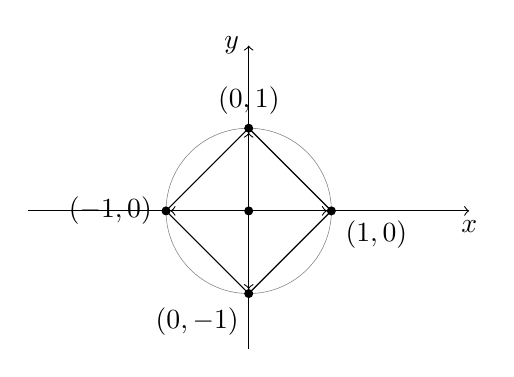
\begin{tikzpicture}[scale=.7,dot/.style={draw,fill,circle,inner sep=1pt}]
  \draw[->] (-4,0) -- (4,0) node[below] {$x$};
  \draw[->] (0,-2.5) -- (0,3) node[left] {$y$};
  \draw[help lines] (0,0) circle (1.5);

  \node[dot,label={below right:$$}] (O) at (0,0) {};
  \foreach \i in {1,...,1} {
        \node[dot,label={\i*360/\m-(\i==\m)*45:$(0,1)$}] (w\i) at (\i*360/\m:1.5) {};
    \draw[->] (O) -- (w\i);
  }
  
  \foreach \i in {4,...,4} {
        \node[dot,label={\i*360/\m-(\i==\m)*45:$(1,0)$}] (w\i) at (\i*360/\m:1.5) {};
    \draw[->] (O) -- (w\i);
  }
  
   \foreach \i in {2,...,2} {
        \node[dot,label={\i*360/\m-(\i==\m)*45:$(-1,0)$}] (w\i) at (\i*360/\m:1.5) {};
    \draw[->] (O) -- (w\i);
  }
  
  \foreach \i in {3,...,3} {
        \node[dot,label={\i*360/\m-(\i==\m)*45:$(0,-1)$}] (w\i) at (\i*360/\m:1.5) {};
    \draw[->] (O) -- (w\i);
  }
  \draw (-1.5,0) -- (0,1.5) -- (1.5,0) -- (0,-1.5) -- (-1.5,0);
    %\draw[-] (w\i) -- (w\j);
 % \draw[->] (0:.3) arc (0:360/\n:.3);
 % \node at (360/\n/2:.5) {$2\pi/5$};
\end{tikzpicture}
\end{center}

Rotations: $\begin{pmatrix}  %0
1 & 0 \\ 0 & 1	
\end{pmatrix}
, \begin{pmatrix}  %\pi/2
0 & -1 \\ 1& 0	
\end{pmatrix}
, 
\begin{pmatrix}		% \pi
-1 & 0 \\ 0 & -1
\end{pmatrix}
,
\begin{pmatrix}  %3\pi/2
0 & 1 \\ -1& 0	
\end{pmatrix}$\\

Angles:\hspace*{30pt} $0$ \quad\quad\quad\hspace*{3pt} $\pi/2$ \quad\quad\quad\hspace*{3pt} $\pi$ \quad\quad\quad\hspace*{3pt} $3\pi/2$\\

Reflections: $\begin{pmatrix}  %0
1 & 0 \\ 0 & -1	\end{pmatrix}
, \begin{pmatrix}  %\pi/2
-1 & 0 \\ 0& 1	
\end{pmatrix}
, 
\begin{pmatrix}		% \pi
0 & 1 \\ 1 & 0     %<--- 
\end{pmatrix}
,
\begin{pmatrix}  %3\pi/2
0 & -1 \\ -1& 0	 %<- 
\end{pmatrix}$
\end{example}


 
 \vspace*{2cm}

\begin{center}
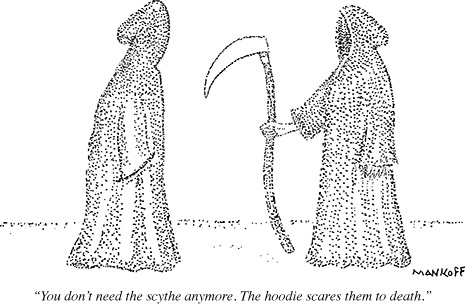
\includegraphics[width = 10cm]{cartoon2.jpg}	
\end{center}


 


 
 

  \sektion{Ring Theory}
    \setcounter{equation}{128}
    
 Many  \lecturemarker{24}{10/03}
of the sets we've looked at so far have \emph{two} binary operations, $+$ and $\times$. We may be interested in studying both at the same time. For instance we might want to look at structures where equations like $x^2 + 1 = 2$, or $y^3 = x^2 + 2$ make sense, which involve both $+$ and $\times$.\\
 
\begin{definition} A \emph{ring}\index{Ring} is a set $R$ with two binary operations $+$ and $\times$ such that the following axioms hold:
 \begin{enumerate}
 \item $(R,+)$ is an abelian group.
 \item $(x \times y)\times z = x \times (y \times z)$ for all $x,y,z \in R$. \textsc{[Associativity]}
 \item $x \times (y + z) = (x \times y) + (x \times z)$, and $(x + y) \times z = (x \times z) + (y \times z)$ for all $x,y,z \in R$ \textsc{[Distributivity]} ``multiplication distributes over addition''\\ \vspace*{-10pt}
 
 $R$ is a \emph{ring with unity} if it also satisfies:\\  \vspace*{-12pt}

 \item  There exists $1 \in R$ such that $1 \times x = x \times 1 = x$. \\ \vspace*{-10pt}

$R$ is a \emph{commutative ring} if it also satisfies:\\ \vspace*{-12pt}
\item $x \times y = y \times x$ for all $x,y \in R$.\\ \vspace*{-10pt}

\boxed{\text{In this course, all rings are assumed to be commutative rings with unity.} }
 \end{enumerate}
 \end{definition}\vspace*{10pt}
 
\begin{examples} \begin{enumerate}
 \item $\Z, \Q, \mathbb{R}, \C$ with their usual $+$ and $\times$.
 \item $\mathbb{Z}_n$ for any $n > 0$, with $+$ and $\times$ defined on residue classes as before.
 \item A non-commutative ring (so Axiom 5 fails): Let $n >1$ and let $R =$ Mat$_n(\mathbb{R})$, the set of all $n \times n$ real matrices with the usual $+$ and $\times$.	
 \end{enumerate}
 \end{examples}\vspace*{10pt}

 
\begin{remarks}~ \begin{enumerate}
 \item We write $0$ for the identity of $(R,+)$.
 \item We can write $x.y$ or $xy$ for $x \times y$.
 \item Fact: $0x = 0$ for any $x \in R$. \begin{proof}
 $0x = 0x + 0$. But $0x = (0 + 0)x = 0x + 0x$ by Distributivity.	 So $0x + 0 = 0x + 0x$. Hence $0x = 0$ by left cancellation in $(R,+)$.
 \end{proof}
 \item It is possible to have a ring $R$ in which $0 = 1$. But in this case $R$ only has one element. This ring is the \emph{trivial ring}. We have seen it before - it is $\Z_1 = \{[0]_1\}$.
 \item The axioms do not say that multiplicative inverses exist. In fact if $R$ is non-trivial, then it has at least one element with no inverse, since $0$ is such an element.\begin{proof}
$0x = 0$ for any $x$. So $0x \neq 1$ for any $x$ unless $0 = 1$. But in this case $R$ is trivial.
\end{proof}
 \end{enumerate}
 \end{remarks}\vspace*{10pt}
 
\begin{definition}

 Let $F$ be a field (e.g. $\mathbb{R}$). The \emph{polynomial ring} $F[x]$ is the set of all polynomials in $x$ with coefficients from $F$, with the usual $+$ and $\times$ for polynomials. Example: $f_1(x)= x^2 + 1$, $f_2(x) = x-3$.
 \[(f_1 + f_2)(x) = x^2 + x -2 \quad (f_1f_2)(x) = x^3 -3x^2 + x -3\]\end{definition} \vspace*{5pt}
 
\begin{definition}
 A non-zero polynomial $f(x)$ has a \emph{degree}\index{Degree}, which is the largest power of $x$ occurring in $f(x)$. Write deg $f(x)$ for the degree. Then we have deg $f(x) \geq 0$ for all $f(x)$. deg $f(x) = 0$ if and only if $f(x)$ is a non-zero constant polynomial.\end{definition} \vspace*{5pt}
 
 We do not define the degree of the zero polynomial $f(x) = 0$. (People who do define it to be $-\infty$)\\
 
 \textit{Exercise:} Show that $F[x]$ is indeed a ring.\\
 
\begin{definition} Let $R$ be a ring with unity. A \emph{unit} in $R$ is an element $u$ such that there exists $w \in R$ with $uw = wu = 1$. So a unit in $R$ is an element with a multiplicative inverse.\end{definition} \vspace*{5pt}
 
\begin{examples}\begin{enumerate}
 \item If $R$ is $\Q,~\mathbb{R},~\C$, then all of its non-zero elements are units.	
 \item If $R = \Z$, then the units are $\{\pm 1\}$.
 \item If $p$ is prime and $R = \Z_p$, then all non-zero elements are units, since $\Z_p^*$ is a group under $\times.$
 \item  
Let   \lecturemarker{25}{11/03} $R = \Z_m$, with $n \neq 1$ and $n$ is not prime. The units in $\Z_m$ are the residue classes $[x]_m$ for $x \in \Z$ such that hcf$(x,m) =1$ (if hcf$(a,b) =1$, we say that $a,b$ are \emph{coprime}\index{Coprime})
 \begin{proof}
 Suppose that $[x]_m$ is a unit in $\Z_m$. Then there exists $[y]_m \in \Z_m$ such that $[x]_m[y]_m = [y]_m[x]_m = [1]_m$. But $[x]_m[y]_m = [xy]_m$, and so $xy \equiv 1 \mod m$. Hence $xy -1 = km$ for some $k\in \Z$. Now $xy - km = 1$. But $xy-km$ is divisible by hcf$(x,m)$. Hence hcf$(x,m) = 1$.\\
 
 Conversely, suppose hcf$(x,m) = 1$. Then Euclid's Algorithm tells us that there exists $y,z \in \Z$ such that $xy + mz = 1$. Now $xy \equiv 1 \mod m$ so $[x]_m[y]_m = [xy]_m = [1]_m$. Hence $[x]_m$ is a unit in $\Z_m$.	
 \end{proof}

\item What are the units in $F[x]$, where $F$ is a field? \\
\textit{Observation:} Let $f_1(x)$, $f_2(x)$ be non-zero polynomials. Then deg $(f_1(x) \times f_2(x)) =$ deg $f_1(x)~ +$ deg $f_2(x)$. In particular, it follows that deg $(f_1(x) \times f_2(x)) \geq$ deg $f_1(x)$.\\

Suppose that $f_1(x)$ is a unit in $F[x]$. Then there exists $f_2(x)$ such that $f_1(x) \times f_2(x) = 1$. So deg $f_1(x) \leq$ deg $1 = 0$. Hence deg $f_1(x) = 0$. Hence $f_1(x)$ is a constant polynomial.\\

Conversely if $f_1(x) = c$, a non-zero constant polynomial, then $f_2(x) = 1/c$ is an inverse for $f_1(x)$. So $f_1(x)$ is a unit. We have shown that units in $F[x]$ are precisely the non-zero constant polynomials.

\item A non-commutative example - the units in the ring Mat$_n(F)$. $(n \times n$ matrices over $F$) are the invertible matrices. There are the elements of $GL_n(F)$. 

 \end{enumerate}\end{examples}\vspace*{5pt}
 
\begin{definition} Given a ring $R$ with unity, we write $R^{\times}$ for the set of units in $R$.	
\end{definition}\vspace*{10pt}
 
\begin{theorem} For any ring $R$ with unity, $(R^{\times},\times)$ is a group. [Called the unit group of $R$.]	
\end{theorem}

 \begin{proof}
First check that $\times$ gives a binary operation on $R^{\times}$. Suppose that $u_1,u_2 \in R^{\times}$. Then there exists $w_1,w_2 \in R^{\times}$ such that $u_1w_1 = w_1u_1 = 1$ and $u_2w_2 = w_2u_2 = 1$. $(u_1u_2)(w_1w_2) = u_1(u_2w_2)w_1 = u_11w_1 = u_1w_1 = 1$. Also $(w_2w_1)(u_1u_2) = w_2(w_1u_1)u_2 = w_21u_2 = w_2u_2 = 1$. So $w_2w_1$ is an inverse for $u_1u_2$, and so $u_1u_2 \in R^{\times}.$\\

Now check the group axioms:

\textsc{Associativity} is given by the ring axioms.

\textsc{Identity:} 1 is a unit since $1\times 1 = 1$. So we have an identity in $R^{\times}$

\textsc{Inverses:} Let $u \in R^{\times}$. Then $u$ has an inverse $w$ in $R$. So $uw = wu = 1$. Now $u$ is an inverse for $w$, and so $w \in R^{\times}$. Hence $u$ has an inverse in $R^{\times}$.
 \end{proof}
 
  \textit{Remarks:}\begin{enumerate}
\item  The proof of Theorem 136 did not assume that $R$ is commutative.
\item Since all units lie in $R^{\times}$, and since any inverse to a unit is itself a unit, it follows that every unit in $R$ has a \emph{unique} inverse. (since this is true in the unit group.) So we can write $u^{-1}$ for the inverse of the unit $u$.
 \end{enumerate}\vspace*{5pt}
 
\begin{examples}\begin{enumerate}
 \item If $R$ is Mat$_n(F)$, then the unit group is $GL_n(F)$. 
 \item If $R$ is $\Q, ~\mathbb{R},~ \C,$ or $\Z_p$ where $p$ is prime, then $R^{\times} = R^* = R \backslash\{0\}$.
 \end{enumerate}
\end{examples}\vspace*{5pt}
 
\begin{definition} A \emph{field}\index{Field} is a commutative ring, $F$, such that $F^* =  F\backslash\{0\}$ (Every non-zero element is a unit.)	
\end{definition}
 
 \subsektion{Arithmetic of Rings}\vsp

\begin{definition} Let $R$ be a ring. Let $a,b \in R$. Say that $a$ \emph{divides} $b$ if there exists $c \in R$ such that $ac = b$. We write $a ~|~ b$ to mean that $a$ divides $b$.	
\end{definition}\vspace*{10pt}

\begin{examples} \begin{enumerate}
 \item If $R = \Z$ then ``$a$ divides $b$'' means what we expect it to.
 \item If $R = \Q,~\mathbb{R},\C$ or any other field, then $a ~|~ b$ for any $a,b \in R$, except when $a = 0$ and $b \neq 0$.
 \item In a polynomial ring $F[x]$, ``divides'' means what it ought to. For example $x -1$ divides $x^2 -2x + 1$ in $\Q[x]$.
 \end{enumerate}
\end{examples}

 
 
 
\begin{proposition} \lecturemarker{26}{13/03}
\begin{enumerate}
 \item  If $a ~|~ b$ then $a ~|~ bc$ for all $c \in R$.
 \item If $a ~|~ b$ and $a ~|~ c$ then $a ~|~ b + c$
 \item If $a ~|~ b$ and $b ~|~ c$ then $a ~|~ c$.
 \item If $u \in R$ is a unit, then $u ~|~ b$ for all $b\in R$.
 \item If $a~|~b$ and if $u$ is a unit, then $au ~|~ b$.
 \item If $u$ is a unit and $w ~|~ u$ then $w$ is also a unit.
 \item $a~|~ 0$ for any $a \in R$.
 \item If $0~|~b$ then $b = 0$.
 \end{enumerate} \end{proposition}(\textit{Proof.} Left as exercise)\\
 
 
 \begin{definition}Let $R$ be a ring, and $r \in R$. We say that $r$ is a \emph{zero-divisor}\index{Zero-divisor} if $\exists s \in R$ such that $s \neq 0$, and $rs = 0$. A ring $R$ with no zero-divisors, apart from $0$, is called an \emph{integral domain}\index{Integral Domain}.
	 \end{definition}\vspace*{10pt}

\begin{examples}\begin{enumerate}
 \item $\Z,~\Q,~\mathbb{R},~\C,~\Z_p$ ($p$ prime), $F[x]$ (where $F = \Q,~\mathbb{R},~\C)$ are all integral domains.
 \item If $m >1$, and $m$ is not prime, then $\Z_m$ is \emph{not}  an integral domain, since if we have $m = ab$, $1<a<m$, then $[a]_m$ and $[b]_m$ are non-zero, but their product is $[m]_m = [0]_m$, and so $[a]_m$ has a zero-divisor.\\
 \end{enumerate}\end{examples}\vspace*{5pt}

\begin{proposition}A unit in a ring $R$ is not a zero-divisor (unless $R$ is trivial.)	
\end{proposition}

 \begin{proof}
 	Let $u$ be a unit. Suppose that $ua = 0$ for some $a \in R$. Then $u^{-1}(ua) = u^{-1}0 = 0$. So (since $u^{-1}(ua) = 1a = a$) we have $a = 0$. Hence $u$ is not a zero-divisor
 \end{proof}
 
  \textbf{Corollary 145.} Any field is an integral domain.
 \begin{proof}
 All non-zero elements in a field are units, and so they are not zero-divisors.  	
 \end{proof}\vspace*{10pt}

 

\begin{proposition} Let $R$ be an integral domain. Let $a,b \in R$ be such that $a ~|~ b$ and $b ~|~ a$. Then there exists a unit $u\in R$ such that $b = au$. %non ID's => \not\exists	
\end{proposition}

\begin{proof}
	Since $a~|~b$, there exists $c \in R$ with $b = ac$. And since $b~|~a$, there exists $d \in R$ such that $a = bd$. $(ac)d = bd = a$, and by associativity it follows that $a(cd) = a$. %not in a group, no cancellation 
	Hence $a(1-cd) = 0$. So one of $a$ or $1-cd = 0$. If $a = 0$, then $b = 0$ since $a~|~ b$, so $a.1 = b$. If $1-cd = 0$, then $cd = 1$, and so $d$ is an inverse for $c$, so $c$ is a unit, with $b = ac$.
\end{proof}\vspace*{10pt}

\begin{definition} Let $R$ be an integral domain. Let $r$ be a non-zero, non-unit in $R$. We say that $r$ is \emph{irreducible}\index{Irreducible} if it can't be written as $r = st$, where $s,t \in R$, and neither $s$ nor $t$ is a unit. Otherwise $r$ is \emph{reducible.}	
\end{definition}
\vspace*{10pt}

\begin{examples}\begin{enumerate}
 \item In $\Z$ the irreducible elements are the primes (positive and negative). Note that if $p$ is prime then $p$ has two factorisations, $p = 1\times p = (-1) \times (-p)$. Here $1$ and $-1$ are the units in $\Z$.
 \item In a field there are no irreducible (or reducible) elements, since every element is either $0$ or a unit.
 \item $f(x) = x-3$ is irreducible in $\Q[x]$ or $\mathbb{R}[x]$ or $\C[x]$. %=> a deg 0 => unit
 \item $f(x) = x^2 -2$ is irreducible in $\Q[x]$. But in $\mathbb{R}[x]$ or $\C[x]$, $f(x)$ is reducible since $x^2 - 2 = (x-\sqrt{2})(x + \sqrt{2})$, and neither of these factors are units.
 \item $f(x) = x^2 + 1$ is irreducible in $\Q[x]$ and $\mathbb{R}[x]$, but is reducible in $\mathbb{C}[x]$ as $x^2 + 1 = (x + i)(x -i)$.
 \end{enumerate}
 \end{examples}

 \textit{Remark.} In an integral domain, every element is exactly one of: zero, a unit, irreducible or reducible. \\

\begin{proposition} Let $F$ be $\Q,~\mathbb{R},~\C$ and let $f(x) \in F[x]$. Let $a \in F$. Then $f(a) = 0$ if and only if $x -a ~|~ f(x).$	
\end{proposition}

\begin{proof}
  \lecturemarker{27}{17/03}

Suppose that $x-a ~|~ f(x)$. Then $f(x) = (x-a)g(x)$, for some $g(x) \in F[x]$. Now $f(a) = (a-a)g(a) = 0$. \\ \vspace*{-5pt}

 For the converse, suppose that $f(a) = 0$. Let $f(x) = \alpha_0 + \alpha_1x + \dots + \alpha_nx^n$, where $\alpha_0, \dots, \alpha_n \in F$. Then $f(x) - f(a) = (\alpha_0 - \alpha_0) + (\alpha_1x -  \alpha_1a) + \dots +(\alpha_nx^n - \alpha_na^n)= \alpha_1(x-a) + \alpha_2(x^2 - a^2) + \dots + \alpha_n(x^n -\alpha^n).$ \\

Note that $x^k = a^k = (x-a)(x^{k-1}+ x^{k-2}a + \dots a^{k-1})$. So $x-a$ divides $x^k - a^k$ for all $k \in \mathbb{N}$. Hence $x-a$ divides $f(x) - f(a)$. But $f(a) = 0$ by assumption, and so $x-a$ divides $f(x)$.
\end{proof}


\begin{theorem}[Fundamental Theorem of Algebra] \index{Fundamental Theorem of Algebra} Let $f(x)\in \C[x]$ be a polynomial of degree greater than 0. Then $f(x)$ has a root in $\C$. (So there exists $a \in \C$ such that $f(a) = 0$.)	
\end{theorem}\vspace*{5pt}

 \textit{Proof. }
Next year's Complex Analysis course.	\\

\begin{corollary}The irreducible elements in $\C[x]$ are the linear polynomials, $\alpha_1x + \alpha_0$, where $\alpha_1 \neq 0$.	
\end{corollary}

\begin{proof}
First show that $\alpha_1x + \alpha_0$ is irreducible. Suppose that $\alpha_1x + \alpha_0 = f(x)g(x)$. Then deg $f(x) +$ deg $g(x) = 1$. So one of $f(x)$ or $g(x)$ has degree $0$, and so is a unit in $\C[x]$. Hence $\alpha_1x + \alpha_0$ is irreducible in $\C[x]$.\\

Conversely, suppose that $r(x)$ has degree $d$ greater than $1$. Then $r(x)$ has a root $a$ by the Fundamental Theorem. So $r(a) = 0$, and so $x-a$ divides $r(x)$ by Proposition 149. So $r(x) = (x-a)s(x)$ for some $s(x) \in \C[x]$. Now deg $s(x) = $ deg $r(x) -1 = d-1 > 0$, so neither $s(x)$ nor $r(x)$ are units in $\C[x]$. So $r(x)$ is reducible. 
\end{proof}\vspace*{5pt}

 \textit{Exercise:} What are the irreducible elements in the ring $\mathbb{R}[x]$?
 \pagebreak

\subsektion{The Rings $\Z[\sqrt{d}]$}\vspace*{5pt}

\begin{definition} Let $d \in \Z$ be a non-square. The ring $\Z[\sqrt{d}]$ is the set $\{x + y\sqrt{d} : x,y \in \Z\} \subseteq \C$, with the usual complex $+$ and $\times$.	
\end{definition}\vspace*{5pt}

Check that these give binary operations on our set:\vspace*{3pt}\\ We have \[(x_1 + y_1\sqrt{d}) + (x_2 + y_2\sqrt{d}) = (x_1 + x_2) + (y_1 + y_2)\sqrt{d} \in \Z[\sqrt{d}]\]
and \[(x_1 + y_1\sqrt{d})(x_2 + y_2\sqrt{d}) = (x_1x_2 + dy_1y_2) + (x_1y_2 + x_2y_1)\sqrt{d} \in \Z[\sqrt{d}]\]
 The ring axioms are left as an exercise.\\

 \textbf{Example:} $\Z[\sqrt{-1}] = \Z[i]$ is the set $\{x + yi : x,y \in \Z\}$, the ring of \emph{Gaussian integers.}\index{Gaussian integers}\\

\begin{proposition} Let $d$ be a non-square in $\Z$. If $x_1 + y_1\sqrt{d} = x_2 + y_2\sqrt{d}$ for $x_1, x_2, y_1, y_2 \in \Z$, then $x_1 = x_2$ and $y_1 = y_2$.	
\end{proposition}

\begin{proof}
Since $d$ is a non-square in $\Z$, we know that $\sqrt{d} \not\in \Q$. Suppose that $x_1 + y_1\sqrt{d} = x_2 + y_2\sqrt{d}$. Then $x_1 - x_2 = (y_2 - y_1)\sqrt{d}$. If $y_2 \neq y_1,$ then $\sqrt{d} = \frac{x_1 - x_2}{y_2 - y_1} \in \Q$, which is a contradiction. So $y_2 = y_1$. Now $x_1 -x_2 = 0$, and so $x_2 = x_1$, as well. 	
\end{proof}\vspace*{5pt}

\begin{definition} Define a function $N: \Z[\sqrt{d}] \to \Z$, by $N(x + y\sqrt{d}) = x^2 - dy^2.$ $N$ is the \emph{norm map}\index{Norm Map} on $\Z[\sqrt{d}].$	
\end{definition}\vspace*{10pt}

\begin{examples}\begin{enumerate}
\item In $\Z[i]$, the norm map is $x + iy \mapsto x^2 + y^2 = |x + iy|^2$.
\item More generally, if $d < 0$, then the norm map is $x+ y\sqrt{d} \mapsto x^2 - dy^2 = x^2 + |d|y^2 = |x + y\sqrt{d}|^2$ (since $x + y\sqrt{d} = x+y\sqrt{|d|}i$).
\item In $\Z[\sqrt{2}]$, the norm map is $x + y\sqrt{2} \mapsto x^2 - 2y^2$. So for example $N(1 + \sqrt{2}) = -1$. When $d > 0$, the norm map can take negative values.
 \end{enumerate}\end{examples}\vspace*{10pt}
 
\begin{proposition}\begin{enumerate}
 \item If $r \in \Z[\sqrt{d}],$ and if $N(r) = 0$, then $r = 0 = 0 + 0\sqrt{d}$
 \item 	If $r,s \in \Z[\sqrt{d}]$, then $N(rs) = N(r)N(s)$.
 \end{enumerate}\end{proposition}
\begin{proof} [Proof (1)] 
Let $r = x + y\sqrt{d}$, and suppose that $N(r) = 0$. Then $x^2 - dy^2 = 0$, and so $x^2 = dy^2$. Now if $y \neq 0$, then $d =\frac{x^2}{y^2} = \left(\frac{x}{y}\right)^2,$ and so $\sqrt{d} \in \Q$. But this is impossible. Hence $y = 0$. Now $N(r) = x^2$, so $x^2 = 0$ and so $x = 0$. Proof of (2) in Homework Sheet.
\end{proof}\vspace*{5pt}



% Recall N(x + y\sqrt{d}) = x^2 -dy^2
\begin{proposition} An   \lecturemarker{28}{18/03}
 element $r$ of $\Z[\sqrt{d}]$ is a unit if and only if $N(r) = \pm 1$. \end{proposition}
\begin{proof}
(only if) Suppose that $r$ is a unit. Then $r$ has an inverse $r^{-1}$. Now $rr^{-1} = 1$, and so $N(r)N(r^{-1}) = N(1)$. But $1 = 1 + 0 \sqrt{d}$, so $N(1) = 1$. Hence $N(r)$ has the inverse $N(r^{-1})$ in $\Z$, so $N(r)$ is a unit in $\Z$. So $N(r) = \pm 1$. \\

(if) Let $r = x + y\sqrt{d}$, and suppose that $N(r) = \pm 1$. Let $s = x - y\sqrt{d}$. Now $rs = x^2 - dy^2 = N(r) = \pm 1$. If $N(r) = 1$ then $s$ an inverse for $r$. If $N(r) = -1$  then $-s$ is an inverse for $r$. In either case, $r$ is a unit in $\Z[\sqrt{d}]$.
\end{proof}\vspace*{5pt}

 \textit{Remark.} If $d = -1$, the $\Z[\sqrt{d}] = \Z[i]$ has $4$ roots, $\pm 1, \pm i$. If $d < -1$, then $\Z[\sqrt{d}]$ has only two units, $\pm 1$. If $d > 0$ then $\Z[\sqrt{d}]$ has infinitely many units.\\

 \textit{Remark.} Elements that are irreducible in $\Z$ [primes] need not be irreducible in $\Z[\sqrt{d}]$.\\

\begin{examples} \begin{enumerate}
 \item $3$ is not irreducible in $\Z[\sqrt{3}]$ since $3 = \sqrt{3} \times \sqrt{3}$, and $\sqrt{3}$ is not a unit.
 \item $2$ is not irreducible in $\Z[i]$, since $2 = (1+i)(1-i)$. 
 \item \textit{Question:} Is $11$ irreducible in $\Z[\sqrt{3}]$?\vspace*{5pt}\\
\textit{Answer:} We have $N(11) = 11^2 = 121$. Suppose that $11 = ab$ in $\Z[\sqrt{-3}]$, where $a$ and $b$ are non-units. $N(a), N(b) \neq \pm 1$. We have $N(a)N(b) = N(11) = 121$. So we must have $N(a) = N(b) = \pm 11$. Since $N$ takes non-negative values on $\Z[\sqrt{-3}]$, we have $N(a) = 11$. Let $a = x + y\sqrt{d}$. Then $x^2 + 3y^2 = 11$. But it is easy to check that no such $x,y$ exist in $\Z$, which is a contradiction. So no such $a,b$ exist. So $11$ is irreducible in $\Z[\sqrt{-3}]$. %+3 harder 
 \end{enumerate}\end{examples}
 
 \subsektion{Highest Common Factor / Greatest Common Divisor}\vsp
\begin{definition} Let $R$ be a ring. Let $a,b,c \in R$. Then $c$ is a \emph{highest common factor}\index{Highest Common Factor} (hcf) or \emph{greatest common divisor} (gcd) for $a$ and $b$ if\begin{enumerate}
\item[(i)] $c ~|~ a$ and $c ~|~ b$	 ~($c$ is a common factor for $a$ and $b$.)
\item[(ii)] If $d ~|~ a$ and $d ~|~ b$ then $d ~|~ c$ for $d \in R$.
\end{enumerate}\end{definition}

 \textit{Remarks.} We do not claim that a highest common factor necessarily exists for all $a,b \in R$. There exists rings $R$ and elements $a,b$ where this doesn't happen. Where hcfs do exist, they are not usually unique. For instance if $R = \Z$, and $a = 4,~ b = 6$, then the hcfs of $a$ and $b$ are $2, -2$. \\

\begin{proposition}Let $R$ be an integral domain. Let $c$ be an hcf for $a$ and $b$ in $R$. Then $d$ is a highest common factor for $a$ and $b$ if and only if $d = cu$, for some unit $u \in R$. 	
\end{proposition}

\begin{proof}
	(only if) Suppose that $c$ and $d$ are both hcfs for $a$ and $b$. So by the 2nd condition in the definition of hcf, we have $c ~|~ d$ and $d ~|~c$. Now by Proposition 146, we have $d = cu$ for a unit $u$. \vspace*{-5pt}\\

	(if) Let $d = cu$, where $u$ is a unit. Since $c ~|~ a$ and $c~|~ b$, we have $cu ~|~ a$ and $cu ~|~ b$, by Proposition 141.5. So $d ~|~ a$ and $d ~|~ b$, so $d$ is a common factor for $a$ and $b$. To show the 2nd hcf condition holds, let $e$ be any common factor of $a$ and $b$. So $e ~|~ a$ and $e ~|~ b$. Then $e ~|~ c$, since $c$ is a hcf. So $e ~|~ cu $ by Proposition 141.3. Hence $e ~|~ d$. Hence $d$ is an hcf for $a$ and $b$.
\end{proof}\vspace*{10pt}


 \textit{Reminder.} Euclids   \lecturemarker{29}{20/03}
 Lemma: If we have any two $a,b\in \Z$, with $b \neq 0$, then there exists $q$ and $r \in \Z$, with  $0 \leq r < |b|$, such that $a = qb + r$.\\


\begin{lemma} Let $f(x)$ and $g(x)$ be polynomials with coefficients from $F,$ $(\Q,,\C)$, with $g(x) \neq 0$. There exist polynomials $q(x)$ and $r(x) \in F[x]$ such that $f(x) = q(x)g(x) + r(x)$, and either $r(x) =0$ or else deg $r(x) <$ deg $g(x)$. 	
\end{lemma}

 \textbf{Example.} Take $F = \Q$, $f(x) = x^4 + x^3 + 2x + 3$ and $g(x) = x^2 -1$. Dividing $f(x)$ by $g(x)$, we get $f(x) = g(x)(x^2 + x + 1) + (3x+4)$. So here $q(x) = x^2 + x + 1$, and $r(x) = 3x + 4$. Here deg $r(x) = 1 < 2 = $ deg $g(x)$.

\begin{proof}[Proof of Lemma 161.]
	Take deg $f(x) = m$ and deg $g(x) = n$. If $m < n$, take $q(x) =0$ and $r(x) = f(x)$, and this satisfies the lemma. So we will assume that $m \geq n$. Now we argue by induction on $m = $ deg $f$. The base case is $m = 0$ (and so $n = 0$ too). $f(x) = a$ and $g(x) = b$ for $a,b \in F$, with $b \neq 0$. Take $q(x) = \frac{a}{b}$, $r(x) = 0$, and this satisfies the lemma.
	
	\textit{Inductive step:} Assume the lemma holds for all polynomials $f(x)$ of degree $<m$. Suppose deg $f(x) = m$. Put \[f(x) = a_mx^m + \dots + a_1x + a_0 \text{ and } g(x) = b_nx^n + \dots + b_1x + b_0\] Define $f'(x) = f(x) - \frac{a_m}{b_n}x^{m-n}g(x)$. The coefficient of $x^m$ in $f'(x)$ is $0$, so deg $f'(x) < m$. So the inductive assumption applies to $f'(x)$, and so there exists $q'(x)$ and $r(x)$ such that $f'(x) = q'(x)g(x) + r(x)$, and with $r(x) = 0$ or deg $r(x) <$ deg $g(x)$.\vspace*{5pt}\\ But now $f(x) = f'(x) + \frac{a_m}{b_n}x^{m-n}g(x) = (q'(x) + \frac{a_m}{b_n}x^{m-n})g(x) + r(x).$ So take $q(x) = q'(x) + \frac{a_m}{b_n}x^{m-n}$, and this satisfies the lemma.
\end{proof}\vspace*{5pt}

 \textbf{Example:} $f(x) = 3x^2 + 5x + 1$, $g(x)= 2x -1$. Calculate $q(x)$ and $r(x)$ using polynomial long division:\\

\polylongdiv{3x^2 + 5x + 1}{2x-1}

So $q(x) = \frac{3}{2}x + \frac{13}{14}, \quad r(x) = \frac{17}{4}$. \\
%Note that leading term of quotient is a_m / b_n, f'(x) is the first remainder

\begin{proposition} Let $R$ be a ring. Let $a,b,q,r \in R$ such that $a = bq + r$. Then $d$ is a highest common factor for $a$ and $b$ if and only if $d$ is a highest common factor for $b$ and $r$.	
\end{proposition}

\begin{proof}
We actually show that the common factors of $a$ and $b$ are the same as those of $b$ and $r$. Suppose $d$ divides $b$ and $r$. Then $d$ divides $bq$ and $r$. So $d$ divides $bq + r = a$. So $d$ divides $a$ and $b$.\\
Conversely, suppose $d$ divides $a$ and $b$. Note that $r = a - bq$. Now $d$ divides $a$ and $bq$, so $d$ divides $a - bq = r$.	
\end{proof}\vspace*{5pt}

 Propositions 161 and 162 give us a Euclidean Algorithm for polynomials. \\

\begin{example}[Euclidean Algorithm for polynomials.] \\$f(x) = x^3 - 2x^2 -5x + 6$, $g(x) = x^2 - 2x -3$.\\
First find $q(x)$ and $r(x)$:\\
\polylongdiv{x^3 - 2x^2 -5x + 6}{x^2 - 2x -3}~

 We have $q(x) = x$, $r(x) = -2x + 6$. Now we look for a hcf of $g(x)$ and $r(x).$ (A ``smaller'' problem than the original.) So applying Euclid's Algorithm again, so now quotient is $-\frac{1}{2}x - \frac{1}{2} ,$ now remainder is $0$. We've shown that $r(x) = -2x + 6$ divides $g(x)$. So $r(x)$ is a hcf for $r(x)$ and $g(x)$. So $r(x)$ is also a hcf for $f(x)$ and $g(x)$ by Proposition 162.

N.B. $-2$ is a unit in $\Q[x]$, with inverse $-\frac{1}{2}$. So $x-3$ is another hcf for $f(x)$ \& $g(x)$.
\end{example}


%What did we need to make Euclid's Algorithm? \begin{itemize}
% \item Prop 162... This holds in any ring.
%\item  Notion of ``smallness'' such that $r$ is ``smaller'' than $b$
% \item Some version of Euclid's Lemma using this notion of `smallness''
%\end{itemize}

\begin{definition} Let  \lecturemarker{30}{24/03}
 $R$ be an integral domain. A \emph{Euclidean function}\index{Euclidean Function} on $R$ is a function $f: R\backslash\{0\} \to \mathbb{N} \cup \{0\}$, which satisfies the following two conditions: \begin{enumerate}
 \item[(i)] $f(ab) \geq f(a)$ for $a,b \in R\backslash\{0\}$
 \item[(ii)] For all $a,b \in R,~b \neq 0$, there exists $q,r \in R$ such that $a = qb + r$, either $r = 0$, or else $f(r) < f(b)$.	
 \end{enumerate}\end{definition}

\begin{examples} \begin{enumerate}
 \item If $R = \Z$ then $f(n) = |n|$ is a Euclidean function. 
 \item If $R = F[x]$ then deg $f(x)$ is a Euclidean function.	
 \end{enumerate}\end{examples}
 \vspace*{5pt}

Euclidean functions are what we need for Euclidean algorithms: \vspace*{5pt}\\
\begin{algorithm}To find a hcf for $a$ and $b$ in a ring $R$ with a Euclidean function $f$.

\textbf{Step 1.} Find $q$ and $r$ such that $a = qb + r$ and $r$ is $0$ or $f(r) < f(b)$

\textbf{Step 2.}	If $r = 0$ then $b$ is a hcf for $a$ and $b$. Otherwise:

\textbf{Step 3.} Start the algorithm again, replacing $a$ with $b$ and $b$ with $r$.

\textit{Since $f(b) \in \mathbb{N}\cup \{0\}$, this algorithm must eventually terminate.}
\end{algorithm}\vspace*{5pt}

\begin{definition} An integral domain with at least one Euclidean function is called a \emph{Euclidean Domain}\index{Euclidean Domain}.\vspace*{5pt}\\
It can be very difficult to decide whether an Integral Domain is Euclidean.
\end{definition}\vspace*{5pt}

Can we find a Euclidean function on $\Z[\sqrt{d}]$? Sometimes!\\

\begin{proposition} Let $d \in \{-2,-1,2,3\}.$ Then the function $f(a) = |N(a)|$ is a Euclidean function on $\Z[\sqrt{d}]$.	
\end{proposition}

\begin{proof}
The first condition from Definition 164 is easy. Since $|N(b)| \geq 1$ for $b \neq 0$, we have $|N(ab)| = |N(a)||N(b)| \geq |N(a)|$.\\

For the second condition, let $a = x + y \sqrt{d}$ and $b = v + w\sqrt{d}$, with $b \neq 0$. In $\C$, calculate: 

\[\dfrac{a}{b} = \dfrac{x + y\sqrt{d}}{v + w\sqrt{d}} = \frac{(x + y\sqrt{d})(v - w\sqrt{d})}{v^2 - dw^2} = \frac{1}{N(b)}((xv-ywd)+(yv-xw)\sqrt{d}).\]
 \[\text{Put ~~ }\alpha = \frac{xv - ywd}{N(b)},~\beta = \frac{yv - xw}{N(b)}, \in \Q\]
 
 Set $m,n$ to be the integers closest to $\alpha,\beta$ respectively. So 
 \[|\alpha - m| \leq \frac{1}{2} \quad \text{and} \quad |\beta - n| \leq \frac{1}{2} \quad (*)\]
 \[\text{Put~~ } q = m + n\sqrt{d} \in \Z[\sqrt{d}] \text{, and } r = a - bq\]
 We show that $|N(r)| < |N(b)|$:\\
 
 Define $c  = N(b)(\frac{a}{b} - q) = N(b)\frac{r}{b} \in \C.$ So $bc = N(b)r$. We have: 
 \[\begin{aligned}
	c &= N(b)(\alpha + \beta \sqrt{d} - m - n\sqrt{d}) \\
	& = N(b)(\alpha - m) + N(b)(\beta - n)\sqrt{d}\\
	& \in \Z[\sqrt{d}], \text{ since } N(b)\alpha \text{ and } N(b)\beta \in \Z
\end{aligned}
 \]
 We have $N(bc) = N(b)N(c) = N(N(b)r) =  N(b)^2N(r)$.\\ 
 
 So $N(c) = N(b)N(r)$. But $N(c) = N(b)^2(\alpha-m)^2 - N(b)^2(\beta-n)^2d$. $N(r) = N(b)(\alpha-m)^2 -d(\beta-n)^2).$\\
 
 Now from $(*)$, $|\alpha-m|$ and $|\beta -n| \leq \frac{1}{2}$. So if $-2 \leq d \leq 3$, it is easy to see that $|(\alpha-m)^2 -d(\beta-n)^2| < 1$. So $|N(r)| < |N(b)|$ as required.
\end{proof}\vspace*{5pt}


  
\begin{example}Find   \lecturemarker{31}{25/03}
a hcf of $a = 4 + \sqrt{2}$ and $b = 2 - 2\sqrt{2}$ in $\Z[\sqrt{2}]$.\\
  
 In $\C$ we calculate: \[\frac{a}{b} = \dfrac{4 + \sqrt{2}}{2 - 2\sqrt{2}} = \dfrac{(4 + \sqrt{2})(2 + 2\sqrt{2})}{(2 - 2\sqrt{2})(2 + 2\sqrt{2})} = -3 - \frac{5}{2}\sqrt{2}\]
 
 So set $q = -3 - 2\sqrt{2}$. ($q = -3-3\sqrt{2}$ would also work.)\\
 
  Now $r = a - bq = 2-\sqrt{2}$. (Notice $|N(r)| = 4 - 2 = 2$, $|N(b)| = |4 - 8| = 4$). Continue, replacing $a$ with $b$ and $b$ with $r$. In $\C$:
 \[\frac{b}{r} = \frac{2-2\sqrt{2}}{2 -\sqrt{2}} = \sqrt{2}\in \Z[\sqrt{2}]\].
 So $q' = -\sqrt{2},~r' = 0$. So $r = 2-\sqrt{2}$ divices $b = 2-2\sqrt{2}$, and so $r$ is a hcf for $b$ and $r$, hence $r$ is a hcf for $a$ and $b$.
 \end{example}\vsp
 
 \begin{lemma} [B\'{e}zout's Lemma] \index{B\'{e}zout's Lemma|idxbf} Let $R$ be a Euclidean domain. Let $a$ and $b$ be elements of $R$ and let $d$ be a hcf for $a$ and $b$. Then there exists $s,t\in R$ such that $as + bt = d$.	
 \end{lemma}

 
 \begin{proof}
 	Define $X = X_{a,b} = \{ax + by : x,y \in R\}$. So $X \subseteq R$. The ring $R$ has a Euclidean function $f$. So if $a$ and $b$ are not both $0$, then $X$ has non-zero elements. So there exists some least $n \in \mathbb{N}\cup\backslash\{0\}$ such that $f(x) = n$ for some $x \in X\backslash\{0\}.$ Let $c$ be some elements of $X \backslash\{0\}$ such that $f(c) = n$. We show that $c$ is a hcf for $a$ and $b$:
 	
 	Since $c = ax + by$ for some $x,y$, it is clear that any common factor of $x$ and $y$ must divide $c$.
 	
 	We know that there exists $q$ and $r\in R$ such that $a = qc + r$, and either $ r = 0$ or $f(r) < f(c)$. Now $c = ax + by$, so $r = a -qc = a - q(ax + by) = a(1-qx) -b(qy) \in X$. We can't have $f(r) < f(c)$, since $f(c)$ is the smallest possible $f$ for elements of $X$. Hence $r = 0$, and so $c~|~ a$. A similar argument shows that $c ~|~ b$, and so $c$ is a common factor - and hence a hcf - for $a$ and $b$.
 	
 	%Proved for some hcf, not all of them 
 	Now let $d$ be any hcf of $a$ and $b$. Then $d =  cu$ for some unit $u \in R$. Now $d = (ax + by)u = axu + byu$. So put $r = xu$ and $s = yu$, and we're done.
 \end{proof}

 
 \subsektion{Unique Factorisation}\vspace*{5pt}
 
\begin{definition}Let $R$ be an integral domain, and let $a,b \in R$. We say $a$ and $b$ are \emph{coprime}\index{Coprime}  if $1$ is a hcf for $a$ and $b$. (Equivalently, any unit is a hcf.)	
\end{definition}\vspace*{5pt}
 
 \begin{proposition} Let $R$ be a Euclidean Domain. Suppose $a$ and $b$ are coprime in $R$, and suppose $a$ divides $bc$. Then $a$ divides $c$.
\end{proposition}

 \begin{proof}
 Since $a ~|~ bc$, we can write $ad = bc$, for some $d \in R$. Since $R$ is Euclidean, and $a$ and $b$ are coprime, we use B\'{e}zout's Lemma: there exist $s,t \in R$ such that $as + bt = 1$. Now $c = 1c = (as + bt)c = asc + btc = asc + (bc)t = asc + (ad)t = a(sc + dt)$, which is divisible by $a$. 
 \end{proof}\vspace*{5pt}
 
 Proposition 172 can fail if $R$ is not Euclidean.
 
 \textbf{Example:} $R = \Z[\sqrt{-3}]$. $a = 2, ~b = 1 + \sqrt{-3},~ c = 1-\sqrt{-3}$. Then $a$ and $b$ are coprime, and $2$ divides $bc = 4$. But $a$ does not divide $c$. (This shows $\Z[\sqrt{-3}]$ is not Euclidean.)\\
 
 \begin{definition} A \emph{unique factorisation domain}\index{Unique Factorisation Domain} is an integral domain $R$ with the following properties:\begin{enumerate}
\item For every $a \in R$, not zero and not a unit, there exists irreducible elements $p_1,\dots,p_s$ in $R$ such that $a = p_1\dots p_s$.
\item Let $p_1,\dots,p_s$ and $q_1,\dots,q_t$ be irreducible in $R$, such that $p_1\dots p_s = q_1\dots q_t$. Then $t = s$, and reordering the $q_i$ if necessary, we have $p_i = q_iu_i$ for some unit $u_i$, for all $i \in \{1,\dots,s\}$. (Factorisation is unique ``up to units''.)
\end{enumerate} \end{definition}

\textit{Example:} $R = \Z$. Then every element except $0,1,-1$ can be written as a product of irreducibles (primes), unique up to sign. $30 = 2\times 3 \times 5 = (-2) \times 3 \times (-5)$.\\

  
 Not   \lecturemarker{32}{27/03}
 every integral domain is a UFD. We've seen that $\Z[\sqrt{-z}]$ is not a UDF.\\
  
\begin{example} In $\Z[\sqrt{-5}]$ we can factorise $6$ as $2\times 3$, and also as $(1 + \sqrt{-5})(1-\sqrt{-5})$. Are these factors irreducible?\vspace*{5pt}\\ We have $N(2) = 4$, $N(3) = 9$. $N(1 \pm \sqrt{-5}) = 6$. If $ab = 2$ or $3$ or $(1 \pm \sqrt{-5})$, and if neither $a$ nor $b$ is a unit, then $N(a)$ must be $\pm 2$ or $\pm 3$. But it is easy to check that the equations $x^2 + 5y^2 = \pm 2$ or $\pm 3$ has no solutions for $x,y \in \Z$. So all of $2,3,1\pm \sqrt{-5}$ are irreducible in $\Z[\sqrt{-5}]$. \vspace*{5pt}\\ Are the factorisations of $6$ the same ``up to units''? No, since $N(2) \neq N(1 \pm \sqrt{-5})$. So $6$ is not uniquely factorisable in $\Z[\sqrt{-5}]$
	
\end{example}

  
  
  \begin{theorem} Every Euclidean Domain is a Unique Factorisation Domain. %converse isn't true\\	
  \end{theorem}

   \textit{Proof.} Omitted. (In Algebra II (?)) 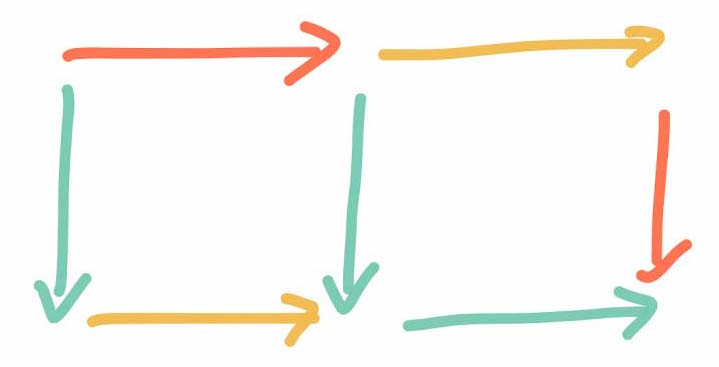
\includegraphics[width=0.08\textwidth]{al2.jpg} 

It follows that $\Z[\sqrt{-5}]$ is not a Euclidean Domain, by Example 174.


\begin{proposition} Let $R$ be a UFD. Let $p$ be an irreducible element of $R$, and let $a,b\in R$ be such that $p ~|~ ab$. Then either $p~|~ a$ or $p~|~ b$.	
\end{proposition}

\begin{proof}
If $a$ or $b$ is $0$ or a unit, then the result is clear. So assume otherwise. So by the first UFD property, there exist irreducible elements $q_1,\dots,q_s$, $r_1,\dots,r_t$, such that $a = q_1\dots q_s$, $b= r_1\dots r_t.$ So $ab = q_1\dots q_s r_1 \dots r_t$.\vspace*{5pt}\\ Now $p~|~ ab$, so $ab = pc$ for some $c \in R$. Suppose that $c = p_1\dots p_u$ as a product of irreducibles. Then $ab = pp_1\dots p_u$. Now by the second (uniqueness) property of UFDs, we have $p = q_iw$ or $r_i w$ for some $i$, and some unit, $w$. If $p = q_iw$ then $p~|~ a$, and if $p = r_1w$ then $p ~|~b$, as required.
\end{proof}\vsp

\begin{definition} A non-unit element, $r$, of a ring $R$ is \emph{prime}\index{Prime} if it has the property that whenever $r ~|~ab$ we have either $r~|~ a$ or $r~|~b$.	
\end{definition}

 \textit{In any integral domain, any prime element is irreducible. Why?}

If $r$ is prime, and $r = ab$, then $r ~|~ ab,$ and then $r~|~ a$ or $r~|~b$ by the prime property. Suppose $r~|~a$. Then since $a ~|~ r$, we have $r = au$ for a unit $u$. So $ab = au$, and so $a(b-u) = 0$. But $R$ is an integral domain, so $b - u =0$. Hence $b = u$, a unit.

In general the converse is not true - we've seen that $2$ is irreducible but not prime in $\Z[\sqrt{-5}]$. (Example 174).\\

\textbf{Felina.} At the start of the Ring Theory section, we mentioned two equations:\begin{enumerate}

\item $x^2 -2 = -1$ we could have solved (in $\Z$) then.
 
\item  The other was $y^3 = x^2 + 2$. \textit{ Can we find all solutions $x,y \in \Z$?}
  \end{enumerate}\vspace*{5pt}
  
  First notice that if $x^2 +2 = y^3$ then both $x$ and $y$ are odd. (It is clear that if one of them is even, then so is the other. Suppose both are even. Then mod $4$, we have $x^2 + 2 \equiv y^3$, and $x^2,y^3 \equiv 0$, so $2 \equiv 0 \mod 4$, a contradiction.)
  
 Move into $\Z[\sqrt{-2}]$. We have $x^2 +2 = (x + \sqrt{-2})(x-\sqrt{-2})$. Put $a = (x+\sqrt{-2})$ and $b = (x-\sqrt{-2}).$ So $y^3 = ab$. Hence $N(y^3) = N(a)N(b).$
 
  Let $d$ the hcf($a,b)$ in $\Z[\sqrt{-2}]$. Then $d$ divides $a-b = 2\sqrt{-2}$. So $N(d)$ divides $N(2\sqrt{-2}),$ so $N(d) $ divides $8$. But $N(d)$ divides $N(a)$, so divides $N(y)^3 = y^6$, which is odd. So $N(d) = 1$.
 
  So hcf$(a,b)$ is a unit, and so $a$ and $b$ are coprime. So we have $y^3 = ab$, where $a,b$ are co-prime. Since $\Z[\sqrt{-2}]$ is a UFD, we can factorise $y^3 = r_1^3 \dots r_t^3$, where $r_1,\dots,r_t$ are irreducible. Now for all $i$, we must have $r_i^3 ~|~ a$ or $r_1^3 ~|~ b$. So it's easy to see that $a=c^3$ and $b = d^3$ for $b,d \in \Z[\sqrt{-2}]$. 
  
  Let $c = m+n\sqrt{-2}$. So $(m + n\sqrt{-2})^3 = x + \sqrt{-2}$. So
  \[(m + n\sqrt{-2})^3  = (m^3 -6mn^2) + (3m^2n-2n^3)\sqrt{-2} = x+\sqrt{-2}\]
  So $m^3 - 6mn^2 = x$ and $3m^2n - 2n^3 = 1$. We have $(3m^2 - 2n^3)n = 1$, so $n~|~1$, hence $n = \pm 1$, and $3m^2 - 2n^2 = n$, so $3m^2 - 2 =\pm 1$. So $n = \pm 1, m = \pm 1$. Now we have $x = \pm 5$. So $x^2 + 2 = 27, y = 3$. So the only solutions are $x = \pm 5, y = 3$.\\
  
  \begin{center}
  \textsf{\textbf{- End of Algebra I -}}	
  \end{center}


 
\end{document}title.jpg